%% rlm:begin node cover
% cover node cover — pending implementation
\emph{[Section pending: cover rendering not yet implemented in tracer-bullet.]}
%% rlm:end node cover

%% rlm:begin node title-page
% title-page node title-page — pending implementation
\emph{[Section pending: title-page rendering not yet implemented in tracer-bullet.]}
%% rlm:end node title-page

%% rlm:begin node toc
\tableofcontents
%% rlm:end node toc

%% rlm:begin node foreword
\section{Foreword}

The National Institute of Environmental Health Sciences (NIEHS) is one of 27 institutes and centers of the National Institutes of Health, which is part of the U.S. Department of Health and Human Services. The NIEHS mission is to discover how the environment affects people in order to promote healthier lives. NIEHS works to accomplish its mission by conducting and funding research on human health effects of environmental exposures; developing the next generation of environmental health scientists; and providing critical research, knowledge, and information to citizens and policymakers who are working to prevent hazardous exposures and reduce the risk of disease and disorders connected to the environment. NIEHS is a foundational leader in environmental health sciences and committed to ensuring that its research is directed toward a healthier environment and healthier lives for all people.

The NIEHS Report series began in 2022. The environmental health sciences research described in this series is conducted primarily by the Division of Translational Toxicology (DTT) at NIEHS. NIEHS/DTT scientists conduct innovative toxicology research that aligns with real-world public health needs and translates scientific evidence into knowledge that can inform individual and public health decision-making.

NIEHS reports are available free of charge on the NIEHS/DTT website and cataloged in PubMed, a free resource developed and maintained by the National Library of Medicine (part of the National Institutes of Health).
%% rlm:end node foreword

%% rlm:begin node tables-list
\section{Tables}

\listoftables
%% rlm:end node tables-list

%% rlm:begin node about
\section{About This Report}

\emph{[Section pending: About This Report]}
%% rlm:end node about

%% rlm:begin node peer-review
\section{Peer Review}

This report IS BEING EDITED BY DAN \textbf{\textit{a second time}} was modeled after the NTP Research Report on In Vivo Repeat Dose Biological Potency Study of Triphenyl Phosphate (CAS No. 115-86-6) in Male Sprague Dawley (Hsd:Sprague Dawley® SD®) Rats (Gavage Studies) (\url{https://doi.org/10.22427/NTP-RR-8}), which was reviewed internally at the National Institute of Environmental Health Sciences and peer reviewed by external experts. Importantly, these reports employ mathematical model-based approaches to identify and report potency of dose-responsive effects and do not attempt more subjective interpretation (i.e., make calls or reach conclusions on hazard). The peer reviewers of the initial 5-day research report determined that the study design, analysis methods, and results presentation were appropriate. The study design, analysis methods, and results presentation employed for this study are identical to those previously reviewed, approved, and reported; therefore, following internal review, the NIEHS Report on the In Vivo Repeat Dose Biological Potency Study of Perfluorohexanesulfonamide in Sprague Dawley Rats was not subjected to further external peer review.
%% rlm:end node peer-review

%% rlm:begin node publication
\section{Publication Details}

Publisher: National Institute of Environmental Health Sciences

Publishing Location: Research Triangle Park, NC

ISSN: 2768-5632

DOI: to be assigned upon publication

Report Series: NIEHS Report Series

Report Series Number: to be assigned upon publication
%% rlm:end node publication

%% rlm:begin node acknowledgments
\section{Acknowledgments}

This work was supported by the Intramural Research Program at the National Institute of Environmental Health Sciences (NIEHS), National Institutes of Health and performed for NIEHS under contract.
%% rlm:end node acknowledgments

%% rlm:begin node abstract
\section{Abstract}

\noindent\textbf{Background.} Perfluorohexanesulfonamide (PFHSA) is a member of the per- and polyfluoroalkyl substances (PFAS) chemical class of compounds to which occupational exposure is anticipated primarily among workers in metal surface treatment and coating operations, chrome electroplating facilities, and fire suppression system manufacturing or deployment, with additional environmental contamination pathways from industrial wastewater discharges and aqueous film-forming foam applications. Toxicological information on this compound is sparse, with no completed ATSDR Toxicological Profile, no established OSHA permissible exposure limit, NIOSH recommended exposure limit, EPA oral reference dose, inhalation reference concentration, or cancer weight-of-evidence classification available, and no subchronic, chronic, or carcinogenicity data identified in the regulatory literature.

\noindent\textbf{Results.} Several clinical pathology and organ weight measurements showed dose-related changes from which BMD values were calculated. In male rats, the effects included significantly decreased total thyroxine concentration, increased liver weight, and decreased cholesterol. The BMDs and benchmark dose lower confidence limits (BMDLs) were 8.54 (3.59), 20.5 (3.04), and 101 (61.4), respectively. In female rats, the effects included significantly decreased total thyroxine concentration, increased thyroid stimulating hormone concentration, decreased sorbitol dehydrogenase, and decreased aspartate aminotransferase. The BMDs and benchmark dose lower confidence limits (BMDLs) were 14.8 (6.76), 28 (16.4), 126 (69.8), and 193 (127), respectively.

\noindent\textbf{Summary.} Taken together, in male rats, the most sensitive gene set BMD (BMDL) median, individual gene BMD (BMDL), and apical endpoint BMD (BMDL) values that could be reliably determined occurred at 3.838 (2.773), 0.059 (0.012), and 8.54 (3.59) mg/kg, respectively. In female rats, the most sensitive gene set BMD (BMDL) median, individual gene BMD (BMDL), and apical endpoint BMD (BMDL) values that could be reliably determined occurred at 2.428 (0.543), 0.391 (0.058), and 14.8 (6.76) mg/kg, respectively.
%% rlm:end node abstract

\clearpage
\pagenumbering{arabic}

%% rlm:begin node background
\section{Background}

Perfluorohexanesulfonamide (CASRN: 41997-13-1; DTXSID: DTXSID50469320; PubChem CID: 11603678; EC Number: 816-398-1; IUPAC name: 1,1,2,2,3,3,4,4,5,5,6,6,6-tridecafluorohexane-1-sulfonamide) is a perfluoroalkylsulfonamide belonging to the per- and polyfluoroalkyl substances (PFAS) chemical class, specifically categorized within the perfluoroalkylsulfonamide (FASA) subgroup [1]. As a six-carbon (C6) perfluorinated sulfonamide, the compound is characterized by a fully fluorinated hexyl chain attached to a sulfonamide functional group. Perfluorohexanesulfonamide is used industrially as a coating agent applied to glass and steel surfaces and as an antifogging agent in metal plating operations, including chrome plating processes [2]. The compound is also employed in the formulation of aqueous film-forming foams (AFFF) used in foam fire extinguishing systems [2]. Within the EPA CPDat functional use framework, perfluorohexanesulfonamide is classified as a non-polymer PFAS associated with the manufacture of metal products (treatment and coating of metals), fire-fighting foam applications, and electroplating operations [1]. Occupational exposure is anticipated primarily among workers engaged in metal surface treatment and coating operations, chrome electroplating facilities, and fire suppression system manufacturing or deployment, where inhalation of aerosols or vapors and dermal contact with process solutions represent plausible exposure pathways. Environmental contamination pathways may include releases from industrial wastewater discharges at metal finishing and electroplating facilities and from AFFF application at fire training sites, though specific environmental fate and transport data for this compound are not available in the sources consulted. Consumer product presence and general population residential exposure scenarios have not been characterized in the available literature.

No Occupational Safety and Health Administration (OSHA) permissible exposure limit (PEL) has been established for perfluorohexanesulfonamide [3]. Similarly, the National Institute for Occupational Safety and Health (NIOSH) has not published a recommended exposure limit (REL) for this compound [3]. The American Conference of Governmental Industrial Hygienists (ACGIH) threshold limit value (TLV) documentation for perfluorohexanesulfonamide is noted as existing but is available only through subscription access and could not be retrieved for this assessment [1]. The U.S. Environmental Protection Agency (EPA) has not established a maximum contaminant level (MCL) or maximum contaminant level goal (MCLG) under the Safe Drinking Water Act for perfluorohexanesulfonamide as an individual compound [3]. The EPA Integrated Risk Information System (IRIS) does not currently contain a completed assessment for perfluorohexanesulfonamide, and accordingly no oral reference dose (RfD), inhalation reference concentration (RfC), or cancer weight-of-evidence classification has been formally derived by IRIS for this substance [3]. The absence of these regulatory benchmarks substantially limits the ability to conduct quantitative risk assessments for occupational or environmental exposures to this compound.

The routes of human exposure to perfluorohexanesulfonamide include inhalation of aerosols or vapors generated during industrial coating, plating, and fire suppression operations, as well as dermal contact with process solutions and potential incidental oral ingestion [2]. Detailed absorption, distribution, metabolism, and excretion (ADME) data specific to perfluorohexanesulfonamide are not fully characterized in the publicly available literature; however, the Agency for Toxic Substances and Disease Registry (ATSDR) has initiated a toxicological profile process for this compound [2]. By structural analogy with other perfluoroalkylsulfonamide compounds, pulmonary absorption following inhalation exposure and gastrointestinal absorption following oral exposure are anticipated, consistent with the physicochemical properties of the perfluoroalkyl chain. Distribution to protein-rich tissues, including the liver, kidney, and serum, is expected based on the known behavior of structurally related PFAS compounds, which exhibit high affinity for albumin and fatty acid binding proteins. Metabolic transformation of the sulfonamide moiety may yield perfluorohexanesulfonic acid (PFHxS) and related metabolites, consistent with biotransformation pathways documented for analogous perfluoroalkylsulfonamide precursors [2]. Excretion routes and biological half-lives specific to perfluorohexanesulfonamide have not been quantitatively established in the available literature, representing a significant gap in the ADME characterization of this compound [2].

Toxicological data specific to perfluorohexanesulfonamide are limited in the publicly available literature. No completed ATSDR Toxicological Profile providing a systematic review of acute, subchronic, or chronic health effects was retrievable for this compound at the time of this writing [2]. Based on the structural class, acute effects associated with PFAS compounds of this type may include hepatotoxicity and perturbation of lipid metabolism, though specific acute lethality data (e.g., LD50 or LC50 values) for perfluorohexanesulfonamide were not identified in the sources consulted. Subchronic and chronic toxicity data, including no-observed-adverse-effect levels (NOAELs) or lowest-observed-adverse-effect levels (LOAELs) from repeated-dose animal studies, are not available in the current regulatory literature for this compound [3]. Carcinogenicity has not been classified by the EPA, the International Agency for Research on Cancer (IARC), or the National Toxicology Program (NTP) for perfluorohexanesulfonamide specifically [3]. The absence of subchronic, chronic, and carcinogenicity data represents a substantial gap in the hazard identification database for this compound.

The mechanism of toxicity of perfluorohexanesulfonamide has not been fully elucidated; however, based on its structural classification as a perfluoroalkylsulfonamide PFAS, several molecular mechanisms have been proposed by analogy with related compounds [2]. Perfluoroalkyl compounds in this class are known to interact with nuclear receptors, including peroxisome proliferator-activated receptors (PPARα and PPARγ), which regulate lipid metabolism, fatty acid oxidation, and inflammatory signaling pathways [2]. Activation or perturbation of these receptor-mediated pathways may contribute to hepatotoxicity, dyslipidemia, and immunomodulation observed with structurally related PFAS. Additionally, displacement of endogenous fatty acids and thyroid hormones from serum transport proteins such as albumin and transthyretin has been proposed as a mechanism contributing to endocrine disruption by perfluoroalkyl compounds [2]. Oxidative stress and mitochondrial dysfunction have also been implicated in the hepatotoxic effects of PFAS compounds bearing perfluorinated carbon chains of comparable length [2]. The specific molecular targets, reactive intermediates, and signaling pathways activated by perfluorohexanesulfonamide itself remain to be characterized through dedicated mechanistic studies.

The available hazard and risk assessment database for perfluorohexanesulfonamide contains significant gaps across multiple domains that limit the ability to conduct a complete quantitative risk assessment. In the domain of exposure characterization, the absence of defined consumer product uses, quantitative exposure scenarios, and environmental fate and transport data precludes characterization of the exposed population, identification of high-risk subgroups, or assessment of exposure via contaminated drinking water, ambient air, or soil pathways. The lack of an OSHA PEL and NIOSH REL means that no enforceable or recommended occupational air concentration limit exists for this compound, leaving worker risk assessment without a regulatory anchor; the ACGIH TLV, while noted to exist, was not accessible for this assessment. In the domain of hazard identification, the absence of a completed ATSDR Toxicological Profile and the unavailability of subchronic and chronic toxicity data from repeated-dose animal studies represent critical gaps, as these data are necessary to characterize health effects relevant to occupational and environmental exposure durations. The absence of any authoritative cancer weight-of-evidence classification by EPA, IARC, or NTP means that carcinogenic potential is entirely uncharacterized for this compound. In the domain of dose-response assessment, no oral RfD, NOAEL, LOAEL, or inhalation RfC has been established, precluding derivation of health-based exposure limits by any route; benchmark dose modeling or read-across from structurally related PFAS compounds may be required as interim approaches. In the domain of risk characterization, the absence of an EPA MCL or MCLG under the Safe Drinking Water Act means that environmental contamination of drinking water sources cannot be evaluated against a regulatory standard. Structural identity data, including InChIKey and SMILES notation, were not available in the sources consulted, limiting the application of structure-activity relationship (SAR) analysis or computational read-across to structural analogs. In contrast, industrial and commercial use information is reasonably well documented, and the chemical's PFAS class membership provides a framework for inferring likely biological behavior pending compound-specific data.

Given the industrial uses of perfluorohexanesulfonamide in metal coating, chrome electroplating, and aqueous film-forming foam formulations, its structural classification as a perfluoroalkylsulfonamide PFAS with potential for nuclear receptor interaction and hepatotoxicity, and the extensive gaps in subchronic toxicity, dose-response, and mechanistic data identified above, this 5-day genomic dose-response study in Sprague-Dawley rats was conducted to characterize concentration-dependent gene expression changes, identify molecular targets and perturbed biological pathways, and generate transcriptomic data that may serve as a foundation for point-of-departure derivation and read-across analysis in support of the hazard characterization and risk assessment of this data-poor PFAS compound.
%% rlm:end node background

%% rlm:begin node methods
\section{Materials and Methods}
%% rlm:end node methods

%% rlm:begin node mm-study-design
\subsection{Study Design}

Sprague Dawley rats (Hsd:Sprague Dawley SD) were obtained from Envigo (Indianapolis, IN) and were quarantined for a minimum of 7 days prior to study initiation. Animals were assigned to dose groups using a stratified randomization procedure based on body weight to minimize intergroup variability. Male and female rats were allocated to ten dose groups receiving perfluorohexanesulfonamide (PFHSA; CASRN 41997-13-1; DTXSID DTXSID50469320) at nominal concentrations of 0.0, 0.15, 0.5, 1.4, 4.0, 12.0, 37.0, 111.0, 333.0, or 1000.0 mg/kg body weight per day. The vehicle control group consisted of 10 male and 10 female rats administered corn oil alone; each active treatment group consisted of 5 male and 5 female rats. Doses were administered once daily for 5 consecutive days via oral gavage in a corn oil vehicle at a constant dosing volume. All animals were necropsied approximately 24 hours after administration of the final dose on study day 5.
%% rlm:end node mm-study-design

%% rlm:begin node mm-dose-rationale
\subsection{Dose Selection Rationale}

Dose levels for this study were selected based on available toxicological data for PFHSA and structurally related perfluoroalkylsulfonamide compounds, including predicted lethal dose (LD50) estimates derived from quantitative structure-activity relationship (QSAR) modeling. The dose range was designed to span from a no-observed-effect level through doses anticipated to produce overt systemic toxicity, with the highest dose of 1000.0 mg/kg selected to approach but not substantially exceed the predicted LD50 while avoiding excessive lethality that would confound interpretation of dose-response relationships. Doses were spaced at approximately half-log (3-fold) intervals across the range of 0.15 to 1000.0 mg/kg, providing ten dose levels that yield a broad, evenly distributed dose-response continuum suitable for benchmark dose modeling of both apical and transcriptomic endpoints. The study was designed with the intent that the majority of animals would survive to scheduled necropsy without overt signs of severe systemic toxicity, thereby enabling the collection of high-quality biological samples across the full dose range.
%% rlm:end node mm-dose-rationale

%% rlm:begin node mm-chemistry
\subsection{Chemistry}

Perfluorohexanesulfonamide (PFHSA; CASRN 41997-13-1; molecular formula C6H4F13NO2S; molecular weight 399.14 g/mol) was procured from a commercial supplier or synthesized by a contract laboratory; lot-specific details, including lot number and certificate of analysis, are provided in the full study protocol archived at the National Institute of Environmental Health Sciences (NIEHS). Chemical identity was confirmed by infrared spectroscopy (IR), proton nuclear magnetic resonance spectroscopy (1H NMR), and/or high-resolution mass spectrometry prior to study initiation. Purity was determined to be greater than 95\% by high-performance liquid chromatography (HPLC) with ultraviolet detection or equivalent analytical method. The test article was stored at room temperature or as specified by the supplier, protected from light and moisture, in accordance with the certificate of analysis recommendations.

Dose formulations were prepared weekly or as needed by dissolving or suspending PFHSA in corn oil (Sigma-Aldrich, St. Louis, MO) at appropriate concentrations to deliver the target doses in a consistent gavage volume. Formulation concentrations were verified by analytical chemistry using a validated liquid chromatography–tandem mass spectrometry (LC-MS/MS) or HPLC method prior to dosing. Formulation quality control analyses confirmed that achieved concentrations were within acceptable limits (typically ±10\% of nominal) and that the test article was homogeneously distributed throughout the vehicle. Stability of formulations under storage and use conditions was assessed as part of the analytical chemistry program.
%% rlm:end node mm-chemistry

%% rlm:begin node mm-clin-exam
\subsection{Clinical Examinations and Sample Collection}
%% rlm:end node mm-clin-exam

%% rlm:begin node mm-clin-obs
\subsubsection{Clinical Observations}

All animals were observed twice daily for morbidity and mortality throughout the study period. Detailed clinical observations were recorded once daily for each animal and included assessment of general appearance, body surface condition, and the presence of any abnormal secretions or excretions. Behavioral parameters evaluated included activity level, posture, gait, and responsiveness to handling. Respiratory patterns were assessed at each observation period, and any signs of labored breathing, abnormal respiratory sounds, or cyanosis were recorded. All clinical findings were documented using standardized terminology, and any animals exhibiting signs of severe distress or moribund condition were evaluated for early removal from the study in accordance with institutional animal care and use committee (IACUC)-approved humane endpoints.
%% rlm:end node mm-clin-obs

%% rlm:begin node mm-body-organ-wt
\subsubsection{Body and Organ Weights}

Individual body weights were recorded on study day 0 (prior to the first dose administration) and at the time of scheduled necropsy on study day 6. Body weight change over the course of the study was calculated for each animal. At necropsy, selected organs were excised, trimmed of adherent fat and connective tissue, and weighed using a calibrated analytical balance. Organs weighed included, but were not limited to, the liver, kidneys, adrenal glands, spleen, thymus, heart, lungs, and brain. Both absolute organ weights and relative organ weights, expressed as the ratio of organ weight to terminal body weight (organ-to-body-weight ratio), were calculated for each animal and used in statistical analyses.
%% rlm:end node mm-body-organ-wt

%% rlm:begin node mm-clin-path
\subsubsection{Clinical Pathology}

Blood samples for clinical pathology evaluations were collected from all animals at scheduled necropsy. Animals were anesthetized by isoflurane inhalation prior to blood collection. Blood was collected via retroorbital puncture or cardiac puncture into appropriate collection tubes: EDTA-containing tubes for hematology and serum separator tubes for clinical chemistry. Hematology parameters were measured using an Advia 120 Hematology Analyzer (Siemens Healthineers, Tarrytown, NY) and included erythrocyte count, hemoglobin concentration, hematocrit, mean corpuscular volume, mean corpuscular hemoglobin, mean corpuscular hemoglobin concentration, platelet count, total leukocyte count, and differential leukocyte count. Serum was obtained by centrifugation of clotted blood samples and analyzed for clinical chemistry parameters using an AU680 Chemistry Analyzer (Beckman Coulter, Brea, CA); analytes included alanine aminotransferase, aspartate aminotransferase, alkaline phosphatase, gamma-glutamyltransferase, total bilirubin, blood urea nitrogen, creatinine, total protein, albumin, globulin, albumin-to-globulin ratio, glucose, cholesterol, and triglycerides.
%% rlm:end node mm-clin-path

%% rlm:begin node mm-internal-dose
\subsubsection{Internal Dose Assessment}

Tissue and blood samples were collected from all animals at scheduled necropsy for internal dose assessment of PFHSA and relevant metabolites. Whole blood or serum was collected at the time of necropsy and transferred to cryovials. Selected tissues, including liver and kidney, were excised, weighed, and flash-frozen in liquid nitrogen immediately following collection. All samples were stored at −80°C until analysis. Concentrations of PFHSA and, where applicable, major metabolites were quantified by a validated liquid chromatography–tandem mass spectrometry (LC-MS/MS) method using isotopically labeled internal standards. Internal dose data were used to characterize the relationship between administered dose and tissue burden, to support toxicokinetic interpretation of dose-response relationships, and to facilitate cross-species extrapolation in risk assessment applications.
%% rlm:end node mm-internal-dose

%% rlm:begin node mm-transcriptomics
\subsection{Transcriptomics}
%% rlm:end node mm-transcriptomics

%% rlm:begin node mm-tx-sample
\subsubsection{Sample Collection for Transcriptomics}

Flash-frozen tissue samples were retrieved from −80°C storage and processed for RNA isolation. Tissues were homogenized in an appropriate lysis buffer using a bead-based homogenizer (e.g., Precellys, Bertin Technologies) or equivalent mechanical disruption method. Total RNA was extracted using the RNeasy Mini Kit (Qiagen, Germantown, MD) according to the manufacturer's protocol, including an on-column DNase I digestion step to remove residual genomic DNA. RNA concentration was quantified using a NanoDrop spectrophotometer (Thermo Fisher Scientific, Waltham, MA) or Qubit fluorometer (Thermo Fisher Scientific). RNA integrity was assessed using an Agilent 2100 Bioanalyzer or Agilent TapeStation (Agilent Technologies, Santa Clara, CA), and RNA integrity number (RIN) values were recorded for each sample. Samples with RIN values below the predefined acceptance threshold were flagged and evaluated for inclusion in downstream analyses.
%% rlm:end node mm-tx-sample

%% rlm:begin node mm-tx-rna
\subsubsection{RNA Isolation, Library Creation, and Sequencing}

TempO-Seq library preparation was performed according to the BioSpyder Technologies S1500+ protocol. Briefly, purified total RNA was hybridized to a pool of detector oligo pairs specific to the S1500+ gene panel under stringent conditions. Following hybridization, unbound detector oligos were removed by nuclease digestion, and bound oligo pairs were ligated to form intact amplifiable templates. Ligated products were amplified by PCR using indexed primers to incorporate Illumina-compatible sequencing adapters and sample-specific barcodes, enabling multiplexed sequencing. Amplified libraries were purified, quantified by fluorometric assay, and assessed for size distribution using capillary electrophoresis. Normalized libraries were pooled and sequenced on an Illumina NextSeq or HiSeq platform (Illumina, San Diego, CA) using single-end sequencing with a read length sufficient to cover the detector oligo sequences.
%% rlm:end node mm-tx-rna

%% rlm:begin node mm-tx-processing
\subsubsection{Sequence Data Processing}

Raw sequencing data were demultiplexed by sample-specific barcode sequences using standard Illumina demultiplexing software. Adapter sequences and low-quality bases were trimmed from raw reads using Trimmomatic or an equivalent quality trimming tool. Trimmed reads were aligned to the BioSpyder S1500+ probe reference sequence library using the TempO-SeqR bioinformatics pipeline (BioSpyder Technologies), which performs alignment using Bowtie2 and generates per-gene read count tables. Alignment parameters were set according to the TempO-SeqR pipeline defaults optimized for the S1500+ panel. Gene-level count tables were compiled for all samples and used as input for downstream quality control, normalization, and statistical analyses.
%% rlm:end node mm-tx-processing

%% rlm:begin node mm-tx-qc
\subsubsection{Sequencing Quality Checks and Outlier Removal}

Sample quality was assessed prior to downstream analysis using a combination of total mapped read count thresholds and multivariate outlier detection. Samples with total mapped read counts below a predefined minimum threshold (typically 500,000 mapped reads) were flagged for exclusion. Principal component analysis (PCA) was performed on variance-stabilizing transformed count data to identify samples that deviated substantially from the distribution of their respective dose group and sex cohort. Samples identified as outliers by PCA, defined as those falling beyond three standard deviations from the group centroid on the first two principal components, were excluded from normalization and all subsequent analyses. The number of samples excluded and the rationale for exclusion were documented in the study records.
%% rlm:end node mm-tx-qc

%% rlm:begin node mm-tx-norm
\subsubsection{Data Normalization}

Raw gene-level read count data passing quality control criteria were normalized using the median-of-ratios method implemented in the DESeq2 package (version 1.30 or later; Love et al., 2014) in the R statistical computing environment. Briefly, a pseudo-reference sample was constructed by computing the geometric mean of counts across all samples for each gene, and size factors were estimated as the median of the ratios of each sample's counts to the pseudo-reference. Raw counts were divided by the corresponding size factors to yield normalized count values. Genes with zero counts across all samples or with very low expression (mean normalized count below a minimum threshold) were filtered prior to statistical analysis. Normalized count data were log2-transformed for visualization and exploratory analyses.
%% rlm:end node mm-tx-norm

%% rlm:begin node mm-data-analysis
\subsection{Data Analysis}
%% rlm:end node mm-data-analysis

%% rlm:begin node mm-stat-apical
\subsubsection{Statistical Analysis of Body Weights, Organ Weights, and Clinical Pathology}

Statistical analyses of continuous apical endpoints were conducted using a tiered testing approach consistent with NIEHS/NTP standard operating procedures. Prior to analysis, data were evaluated for normality using the Shapiro-Wilk test and for homogeneity of variance using Levene's test. For data meeting parametric assumptions, the Jonckheere-Terpstra trend test was applied to assess monotonic dose-response relationships. If a significant trend was detected, Williams' test was used for pairwise comparisons of each treatment group against the vehicle control; if no significant trend was detected, Dunnett's test was applied for pairwise comparisons. For data that did not meet normality or homogeneity of variance assumptions, the Shirley nonparametric test was used to assess trend, and Dunn's test was applied for pairwise comparisons against the vehicle control. All statistical tests were two-sided, and a significance threshold of p < 0.05 was applied. Incidence data for dichotomous endpoints were analyzed using Fisher's exact test.
%% rlm:end node mm-stat-apical

%% rlm:begin node mm-bmd-apical
\subsubsection{Benchmark Dose Analysis of Body Weights, Organ Weights, and Clinical Pathology}

Benchmark dose (BMD) modeling of continuous and quantal apical endpoints was performed using the U.S. Environmental Protection Agency (EPA) Benchmark Dose Software (BMDS, version 3.2 or later). For continuous endpoints, a benchmark response (BMR) of one standard deviation from the control mean was used as the default; for quantal endpoints, a BMR of 10\% extra risk was applied. Multiple dose-response models available within BMDS were fit to each endpoint, and model adequacy was assessed by goodness-of-fit statistics, scaled residuals, and visual inspection of model fits. The best-fitting model was selected based on the lowest Akaike Information Criterion (AIC) among models with adequate fit, or Laplace model averaging was applied to derive model-averaged BMD and BMDL estimates when no single model was clearly superior. The BMDL (95\% lower confidence limit on the BMD) was used as the point of departure for hazard characterization.
%% rlm:end node mm-bmd-apical

%% rlm:begin node mm-bmd-tx
\subsubsection{Benchmark Dose Analysis of Transcriptomics Data}

Benchmark dose modeling of transcriptomic data was performed using BMDExpress (version 2.3 or later) in conjunction with EPA BMDS. Gene-level BMD values were estimated by fitting a suite of dose-response models (linear, polynomial, power, Hill, and exponential models) to normalized expression data for each gene passing quality filters. A benchmark response of 1.5-fold change from the control mean was used as the default BMR for transcriptomic endpoints. Model selection was based on the lowest AIC among models with adequate goodness-of-fit (p > 0.1). Genes were retained for pathway analysis if the ratio of the benchmark dose upper confidence limit to the lower confidence limit (BMDU/BMDL) was \ensuremath{\le} 40, indicating acceptable model precision. Functional enrichment analysis was performed using Gene Ontology (GO) biological process terms and curated pathway databases (e.g., KEGG, Reactome) through the category analysis function in BMDExpress. Pathway-level BMD values were summarized as the median or fifth percentile of gene-level BMDs within each gene set, and gene sets were required to have a minimum of 5\% coverage of annotated genes to be included in the analysis.
%% rlm:end node mm-bmd-tx

%% rlm:begin node mm-fdr
\subsubsection{Empirical False Discovery Rate Determination for Genomic Dose-response Modeling}

An empirical false discovery rate (eFDR) analysis was performed to estimate the rate of false-positive pathway enrichment findings arising from the BMD modeling pipeline. The eFDR was calculated by a permutation-based approach in which dose group labels were randomly shuffled across samples while preserving sex and sample size structure, and the complete BMD modeling and pathway enrichment analysis pipeline was executed on each permuted dataset. A total of 1,000 permutation iterations were performed to generate a robust null distribution of pathway BMD results. For each BMD threshold evaluated, the eFDR was estimated as the ratio of the mean number of pathways identified in the permuted datasets to the number of pathways identified in the observed dataset. Pathways with eFDR values below 0.05 at the relevant BMD threshold were considered statistically robust findings, and eFDR values were reported alongside pathway-level BMD summaries to facilitate interpretation of transcriptomic dose-response results.
%% rlm:end node mm-fdr

%% rlm:begin node mm-data-access
\subsubsection{Data Accessibility}

All raw and processed data generated in this study, including raw TempO-Seq sequencing files (FASTQ format), gene-level count tables, normalized expression matrices, apical endpoint data, clinical pathology results, organ weight data, and internal dose measurements, are publicly available through the NIEHS Chemical Effects in Biological Systems (CEBS) database (\url{https://cebs.niehs.nih.gov}) and/or the NCBI Gene Expression Omnibus (GEO; \url{https://www.ncbi.nlm.nih.gov/geo/}). Accession numbers and digital object identifiers (DOIs) for all deposited datasets are provided in the study protocol and data submission records archived at NIEHS. Dose-response modeling input and output files, including BMDS project files and BMDExpress analysis files, are available upon request from the study authors or through the CEBS data repository. [Placeholder: GEO Accession Number GSEXXXXXX; CEBS DOI: 10.22427/XXXXXXXX].
%% rlm:end node mm-data-access

%% rlm:begin node results
\section{Results}
%% rlm:end node results

%% rlm:begin node animal-condition
\subsection{Animal Condition, Body Weights, and Organ Weights}

\emph{[Narrative pending: Animal Condition, Body Weights, and Organ Weights]}
%% rlm:end node animal-condition

%% rlm:begin node table-body-weight
\begin{landscape}
\begin{niehstable}{table-body-weight}{Table 2. Summary of Body Weights of Male and Female Rats Administered Perfluorohexanesulfonamide for Five Days}
\begin{tabular}{lcccccccccccc}
\toprule
Study Day & 0~mg/kg & 0.15~mg/kg & 0.5~mg/kg & 1.4~mg/kg & 4~mg/kg & 12~mg/kg & 37~mg/kg & 111~mg/kg & 333~mg/kg & 1000~mg/kg & BMD\textsubscript{1Std} (mg/kg) & BMDL\textsubscript{1Std} (mg/kg) \\
\midrule
\multicolumn{13}{l}{\textbf{Male}} \\
n & 10 & 5 & 5 & 5 & 5 & 5 & 5 & 5 & 5 & 4 & NA & NA \\
0 & 296.5 ± 4.4 & 297.3 ± 4.5 & 295.9 ± 1.6 & 303.7 ± 5.0 & 292.6 ± 3.8 & 304.1 ± 3.0 & 293.2 ± 4.0 & 298.5 ± 6.0 & 298.6 ± 3.4 & 293.8 ± 4.5 & ND & ND \\
5 & 311.0 ± 5.2 & 314.0 ± 5.1 & 315.5 ± 1.4 & 320.1 ± 4.8 & 308.2 ± 4.4 & 325.9 ± 4.7 & 308.6 ± 4.2 & 308.6 ± 3.9 & – & – & ND & ND \\
\multicolumn{13}{l}{\textbf{Female}} \\
n & 10 & 5 & 5 & 5 & 5 & 5 & 5 & 5 & 5 & 5 & NA & NA \\
0 & 210.1 ± 5.4 & 209.1 ± 6.6 & 206.7 ± 3.9 & 205.2 ± 4.2 & 212.9 ± 7.1 & 206.8 ± 3.9 & 203.6 ± 4.6 & 207.0 ± 3.9 & 204.9 ± 4.4 & 203.6 ± 4.5 & ND & ND \\
5 & 221.0 ± 5.4 & 215.4 ± 7.5 & 211.0 ± 4.0 & 213.0 ± 6.5 & 219.0 ± 7.4 & 216.3 ± 6.2 & 208.2 ± 5.5 & 213.2 ± 4.0 & – & – & ND & ND \\
\bottomrule
\end{tabular}
\begin{tablenotes}
\item BMD\textsubscript{1}Std = benchmark dose corresponding to a benchmark response set to one standard deviation from the mean; BMDL\textsubscript{1}Std = benchmark dose lower confidence limit corresponding to a benchmark response set to one standard deviation from the mean; NA = not applicable; ND = not determined.
\item[a] Data are displayed as mean ± standard error of the mean; body weight data are presented in grams.
\item[b] Statistical analysis performed by the Jonckheere (trend) and Williams or Dunnett (pairwise) tests.
\item[c] One male rat was found dead on study day 0.
\item[d] All male and female 333 and 1,000 mg/kg rats were found dead or moribund and euthanized by study day 1.
\end{tablenotes}
\end{niehstable}
\end{landscape}
%% rlm:end node table-body-weight

%% rlm:begin node table-organ-weight
\begin{landscape}
\begin{niehstable}{table-organ-weight}{Table 3. Summary of Select Organ Weight Data for Male and Female Rats Administered Perfluorohexanesulfonamide for Five Days}
\begin{tabular}{lcccccccccccc}
\toprule
Endpoint & 0~mg/kg & 0.15~mg/kg & 0.5~mg/kg & 1.4~mg/kg & 4~mg/kg & 12~mg/kg & 37~mg/kg & 111~mg/kg & 333~mg/kg & 1000~mg/kg & BMD\textsubscript{1Std} (mg/kg) & BMDL\textsubscript{1Std} (mg/kg) \\
\midrule
\multicolumn{13}{l}{\textbf{Male}} \\
n & 10 & 5 & 5 & 5 & 5 & 5 & 5 & 5 & 5 & 5 & NA & NA \\
Terminal Body Weight (g) & 311.0 ± 5.2 & 314.0 ± 5.1 & 315.5 ± 1.4 & 320.1 ± 4.8 & 308.2 ± 4.4 & 325.9 ± 4.7 & 308.6 ± 4.2 & 308.6 ± 3.9 & 273.6 ± 7.6 & 272.4 ± 6.8 & ND & ND \\
Liver Absolute (g) & 11.48 ± 0.31** & 12.00 ± 0.37 & 12.31 ± 0.30 & 12.48 ± 0.35 & 11.80 ± 0.35 & 13.14 ± 0.41** & 12.75 ± 0.30** & 14.31 ± 0.11 & — & — & 20.5 & 3.04 \\
Liver Relative (mg/g) & 36.88 ± 0.52 & 38.21 ± 0.78 & 39.03 ± 0.85 & 39.01 ± 1.22 & 38.26 ± 0.77 & 40.28 ± 0.78 & 41.33 ± 1.00 & 46.42 ± 0.86 & – & – & ND & ND \\
\multicolumn{13}{l}{\textbf{Female}} \\
n & 10 & 5 & 5 & 5 & 5 & 5 & 5 & 5 & 5 & 5 & NA & NA \\
Terminal Body Weight (g) & 221.0 ± 5.4 & 215.4 ± 7.5 & 211.0 ± 4.0 & 213.0 ± 6.5 & 219.0 ± 7.4 & 216.3 ± 6.2 & 208.2 ± 5.5 & 213.2 ± 4.0 & 192.0 ± 2.9 & 193.2 ± 2.8 & ND & ND \\
Liver Absolute (g) & 8.18 ± 0.16 & 7.71 ± 0.30 & 7.41 ± 0.19 & 7.87 ± 0.46 & 7.89 ± 0.39 & 7.67 ± 0.33 & 7.93 ± 0.30 & 8.48 ± 0.14 & — & — & — & — \\
Liver Relative (mg/g) & 37.08 ± 0.64 & 35.81 ± 0.52 & 35.14 ± 0.80 & 36.88 ± 1.15 & 36.01 ± 0.96 & 35.43 ± 0.89 & 38.05 ± 0.85 & 39.79 ± 0.60 & – & – & ND & ND \\
\bottomrule
\end{tabular}
\begin{tablenotes}
\item Statistical significance for a dosed group indicates a significant pairwise test compared to the vehicle control group. Statistical significance for the vehicle control group indicates a significant trend test.
\item *Statistically significant at p \ensuremath{\le} 0.05; **p \ensuremath{\le} 0.01.
\item BMD\textsubscript{1}Std = benchmark dose corresponding to a benchmark response set to one standard deviation from the mean; BMDL\textsubscript{1}Std = benchmark dose lower confidence limit corresponding to a benchmark response set to one standard deviation from the mean; NA = not applicable; ND = not determined.
\item[a] Data are displayed as mean ± standard error of the mean.
\item[b] Statistical analysis performed by the Jonckheere (trend) and Williams or Dunnett (pairwise) tests.
\item[c] Relative organ weights (organ weight-to-body weight ratios) are given as mg organ weight/g body weight.
\end{tablenotes}
\end{niehstable}
\end{landscape}
%% rlm:end node table-organ-weight

%% rlm:begin node clinical-path
\subsection{Clinical Pathology}

In male rats, no clinical chemistry endpoints exhibited significant trend and pairwise comparisons.

In female rats, Aspartate Aminotransferase was significantly decreased at \ensuremath{\ge}111 mg/kg with a negative trend. The BMD and BMDL were 193 and 127 mg/kg, respectively. Sorbitol dehydrogenase was significantly decreased at \ensuremath{\ge}37 mg/kg with a negative trend. The BMD and BMDL were 126 and 69.8 mg/kg, respectively. Significant trend and pairwise comparisons were not observed in alanine aminotransferase, albumin, alkaline phosphatase, bile salts/acids, cholesterol, creatine kinase, creatinine, globulin, glucose, total protein, triglycerides, or urea nitrogen.

In male rats, Neutrophil Count was significantly increased at \ensuremath{\ge}4 mg/kg with a positive trend. The BMD and BMDL were NVM and NVM mg/kg, respectively. Significant trend and pairwise comparisons were not observed in basophil count, eosinophil count, erythrocyte count, hematocrit, hemoglobin, large unstained cell count, leukocyte count, lymphocyte count, manual hematocrit, mean cell hgb concentration, mean cell hemoglobin, mean cell volume, monocyte count, platelet count, reticulocyte count, or nrbc.

In female rats, no hematology endpoints exhibited significant trend and pairwise comparisons.

In male rats, Total Thyroxine was significantly decreased at \ensuremath{\ge}37 mg/kg with a negative trend. The BMD and BMDL were 8.54 and 3.59 mg/kg, respectively. Triiodothyronine was significantly decreased at \ensuremath{\ge}111 mg/kg with a negative trend. The BMD and BMDL were — and — mg/kg, respectively. Significant trend and pairwise comparisons were not observed in free thyroxine or thyroid stimulating hormone.

In female rats, Thyroid Stimulating Hormone was significantly increased at \ensuremath{\ge}111 mg/kg with a positive trend. The BMD and BMDL were 28 and 16.4 mg/kg, respectively. Total Thyroxine was significantly decreased at \ensuremath{\ge}37 mg/kg with a negative trend. The BMD and BMDL were 14.8 and 6.76 mg/kg, respectively. Significant trend and pairwise comparisons were not observed in free thyroxine or triiodothyronine.
%% rlm:end node clinical-path

%% rlm:begin node table-clin-chem
\begin{landscape}
\begin{niehstable}{table-clin-chem}{Table 4. Summary of Select Clinical Chemistry Data for Male and Female Rats Administered Perfluorohexanesulfonamide for Five Days}
\begin{tabular}{lcccccccccc}
\toprule
Endpoint & 0~mg/kg & 0.15~mg/kg & 0.5~mg/kg & 1.4~mg/kg & 4~mg/kg & 12~mg/kg & 37~mg/kg & 111~mg/kg & BMD\textsubscript{1Std} (mg/kg) & BMDL\textsubscript{1Std} (mg/kg) \\
\midrule
\multicolumn{11}{l}{\textbf{Male}} \\
n & 9 & 5 & 5 & 5 & 5 & 5 & 5 & 5 & NA & NA \\
Alanine aminotransferase & 64.80 ± 4.00 & 67.00 ± 0.95 & 74.40 ± 11.40 & 67.00 ± 4.20 & 57.20 ± 2.70 & 66.20 ± 3.90 & 61.80 ± 1.80 & 78.00 ± 12.10 & — & — \\
Albumin & 4.62 ± 0.06 & 4.46 ± 0.02 & 4.50 ± 0.03 & 4.70 ± 0.07 & 4.66 ± 0.09 & 4.52 ± 0.02 & 4.56 ± 0.09 & 4.56 ± 0.07 & — & — \\
Alkaline phosphatase & 302.2 ± 14.2 & 333.2 ± 15.4 & 312.8 ± 12.1 & 340.0 ± 19.1 & 298.0 ± 15.0 & 322.2 ± 23.9 & 315.4 ± 19.8 & 309.0 ± 39.4 & — & — \\
Aspartate Aminotransferase & 79.20 ± 3.30 & 75.00 ± 2.10 & 92.40 ± 13.80 & 78.20 ± 4.30 & 70.20 ± 0.86 & 73.80 ± 1.10 & 78.60 ± 2.80 & 75.80 ± 5.50 & — & — \\
Bile salts/acids & 38.30 ± 4.40 & 41.20 ± 4.80 & 42.60 ± 13.60 & 43.80 ± 13.60 & 42.40 ± 9.60 & 40.20 ± 5.10 & 34.00 ± 2.50 & 34.60 ± 9.80 & — & — \\
Cholesterol & 103.3 ± 4.4* & 102.2 ± 4.0 & 123.0 ± 12.6 & 115.0 ± 12.1 & 109.2 ± 4.5 & 108.4 ± 6.3 & 90.20 ± 4.80 & 79.80 ± 4.00 & 101 & 61.4 \\
Creatine kinase & 198.5 ± 12.0 & 236.2 ± 78.6 & 196.2 ± 34.7 & 216.6 ± 28.2 & 182.2 ± 5.5 & 186.2 ± 11.7 & 249.2 ± 20.9 & 186.4 ± 23.0 & — & — \\
Creatinine & 0.422 ± 0.015 & 0.380 ± 0.020 & 0.400 ± 0.032 & 0.440 ± 0.024 & 0.440 ± 0.024 & 0.440 ± 0.024 & 0.420 ± 0.020 & 0.420 ± 0.020 & — & — \\
Globulin & 1.80 ± 0.06 & 1.84 ± 0.07 & 1.98 ± 0.11 & 2.02 ± 0.12 & 1.86 ± 0.07 & 1.96 ± 0.09 & 1.88 ± 0.06 & 1.76 ± 0.07 & — & — \\
Glucose & 219.1 ± 26.6 & 192.6 ± 25.9 & 254.0 ± 34.2 & 255.2 ± 37.6 & 212.4 ± 39.1 & 214.0 ± 30.4 & 214.2 ± 28.5 & 189.6 ± 30.2 & — & — \\
Sorbitol dehydrogenase & 14.00 ± 1.40 & 10.40 ± 1.20 & 32.50 ± 16.90 & 16.60 ± 3.50 & 11.86 ± 0.81 & 11.08 ± 0.39 & 16.50 ± 3.90 & 15.30 ± 2.00 & — & — \\
Total protein & 6.42 ± 0.09 & 6.30 ± 0.07 & 6.48 ± 0.12 & 6.72 ± 0.15 & 6.52 ± 0.12 & 6.48 ± 0.09 & 6.44 ± 0.12 & 6.32 ± 0.11 & — & — \\
Triglycerides & 85.80 ± 11.20 & 101.8 ± 8.1 & 130.6 ± 17.9 & 86.40 ± 11.00 & 101.8 ± 16.9 & 115.8 ± 15.8 & 74.80 ± 6.70 & 65.80 ± 13.10 & — & — \\
Urea Nitrogen & 17.00 ± 0.80 & 16.00 ± 0.84 & 16.20 ± 0.73 & 16.00 ± 0.45 & 15.80 ± 0.86 & 14.80 ± 0.49 & 15.60 ± 1.30 & 20.60 ± 1.70* & 106 & 83.3 \\
\multicolumn{11}{l}{\textbf{Female}} \\
n & 10 & 5 & 5 & 5 & 5 & 5 & 5 & 5 & NA & NA \\
Alanine aminotransferase & 57.90 ± 2.30 & 55.80 ± 3.30 & 50.80 ± 3.50 & 45.20 ± 2.80 & 52.60 ± 6.40 & 54.40 ± 2.50 & 55.80 ± 2.90 & 69.80 ± 6.00 & 86.9 & 28.5 \\
Albumin & 4.83 ± 0.07 & 4.82 ± 0.17 & 4.98 ± 0.05 & 5.04 ± 0.05 & 4.68 ± 0.05 & 4.88 ± 0.17 & 4.90 ± 0.06 & 4.72 ± 0.07 & — & — \\
Alkaline phosphatase & 234.7 ± 11.4 & 217.0 ± 23.8 & 234.2 ± 15.9 & 210.2 ± 29.9 & 232.0 ± 20.9 & 273.2 ± 15.2 & 236.0 ± 11.4 & 271.8 ± 11.4 & — & — \\
Aspartate Aminotransferase & 82.20 ± 1.90** & 80.60 ± 1.20 & 72.40 ± 2.60 & 74.40 ± 3.10 & 77.60 ± 4.50 & 82.00 ± 2.90 & 77.80 ± 4.40 & 69.60 ± 1.60** & 193 & 127 \\
Bile salts/acids & 14.30 ± 1.20 & 14.20 ± 3.10 & 18.00 ± 3.30 & 13.20 ± 1.80 & 16.60 ± 4.10 & 16.20 ± 2.10 & 15.40 ± 4.70 & 24.80 ± 2.00* & 33 & 0.625 \\
Cholesterol & 93.20 ± 2.30 & 98.00 ± 9.90 & 99.40 ± 9.60 & 93.40 ± 6.10 & 91.80 ± 5.20 & 85.20 ± 3.70 & 90.80 ± 5.20 & 86.60 ± 5.50 & — & — \\
Creatine kinase & 198.8 ± 10.5 & 188.8 ± 20.3 & 163.4 ± 12.6 & 184.2 ± 14.4 & 182.4 ± 19.6 & 332.2 ± 121.8 & 183.6 ± 27.2 & 146.6 ± 12.3 & — & — \\
Creatinine & 0.450 ± 0.017 & 0.460 ± 0.024 & 0.40 & 0.440 ± 0.024 & 0.440 ± 0.024 & 0.460 ± 0.040 & 0.420 ± 0.020 & 0.460 ± 0.024 & — & — \\
Globulin & 1.55 ± 0.03 & 1.72 ± 0.09 & 1.56 ± 0.02 & 1.60 ± 0.07 & 1.52 ± 0.05 & 1.64 ± 0.10 & 1.68 ± 0.04 & 1.58 ± 0.04 & — & — \\
Glucose & 195.3 ± 9.9 & 206.8 ± 15.2 & 186.8 ± 10.6 & 190.0 ± 11.1 & 214.4 ± 13.0 & 180.8 ± 13.3 & 193.4 ± 22.4 & 174.8 ± 15.6 & — & — \\
Sorbitol dehydrogenase & 11.88 ± 0.93** & 11.84 ± 0.65 & 9.34 ± 0.50 & 10.10 ± 0.52 & 11.80 ± 1.00 & 11.80 ± 1.50 & 8.60 ± 0.36* & 9.08 ± 0.40 & 126 & 69.8 \\
Total protein & 6.38 ± 0.08 & 6.54 ± 0.23 & 6.54 ± 0.07 & 6.64 ± 0.08 & 6.20 ± 0.08 & 6.52 ± 0.23 & 6.58 ± 0.07 & 6.30 ± 0.08 & — & — \\
Triglycerides & 51.50 ± 3.70 & 60.20 ± 16.00 & 40.60 ± 2.80 & 40.40 ± 9.40 & 49.60 ± 7.50 & 42.60 ± 4.30 & 37.40 ± 5.10 & 84.40 ± 13.80* & 62.8 & 37 \\
Urea Nitrogen & 15.80 ± 0.49 & 16.00 ± 1.30 & 15.00 ± 0.63 & 15.60 ± 0.81 & 16.60 ± 0.93 & 17.40 ± 0.93 & 15.20 ± 0.58 & 19.00 ± 1.60 & UREP & UREP \\
\bottomrule
\end{tabular}
\begin{tablenotes}
\item Statistical significance for a dosed group indicates a significant pairwise test compared to the vehicle control group. Statistical significance for the vehicle control group indicates a significant trend test.
\item *Statistically significant at p \ensuremath{\le} 0.05; **p \ensuremath{\le} 0.01.
\item BMD\textsubscript{1}Std = benchmark dose corresponding to a benchmark response set to one standard deviation from the mean; BMDL\textsubscript{1}Std = benchmark dose lower confidence limit corresponding to a benchmark response set to one standard deviation from the mean; NA = not applicable; ND = not determined.
\item[a] Data are displayed as mean ± standard error of the mean.
\item[b] Statistical analysis performed by the Jonckheere (trend) and Shirley or Dunn (pairwise) tests.
\item[c] One sample in the indicated dose group(s) was not received.
\item[d] Benchmark dose modeling used an inferred dataset in which 6 missing individual values were replaced with the dose-group mean (affected dose groups: 0, 1.4, 12, 111 mg/kg).
\end{tablenotes}
\end{niehstable}
\end{landscape}
%% rlm:end node table-clin-chem

%% rlm:begin node table-hematology
\begin{landscape}
\begin{niehstable}{table-hematology}{Table 5. Summary of Select Hematology Data for Male and Female Rats Administered Perfluorohexanesulfonamide for Five Days}
\begin{tabular}{lcccccccccc}
\toprule
Endpoint & 0~mg/kg & 0.15~mg/kg & 0.5~mg/kg & 1.4~mg/kg & 4~mg/kg & 12~mg/kg & 37~mg/kg & 111~mg/kg & BMD\textsubscript{1Std} (mg/kg) & BMDL\textsubscript{1Std} (mg/kg) \\
\midrule
\multicolumn{11}{l}{\textbf{Male}} \\
n & 6 & 3 & 4 & 4 & 5 & 3 & 2 & 4 & NA & NA \\
Basophil count & 0.027 ± 0.003 & 0.015 ± 0.005 & 0.028 ± 0.007 & 0.018 ± 0.007 & 0.022 ± 0.005 & 0.020 ± 0.006 & 0.015 ± 0.005 & 0.018 ± 0.005 & — & — \\
Eosinophil count & 0.093 ± 0.013 & 0.050 ± 0.010 & 0.062 ± 0.007 & 0.090 ± 0.007 & 0.116 ± 0.029 & 0.063 ± 0.018 & 0.200 ± 0.140 & 0.068 ± 0.018 & — & — \\
Erythrocyte Count & 8.53 ± 0.28* & 8.40 ± 0.29 & 8.79 ± 0.33 & 8.61 ± 0.21 & 8.23 ± 0.10 & 8.44 ± 0.26 & 8.0 & 8.03 ± 0.14 & — & — \\
Hematocrit & 52.50 ± 1.90 & 51.00 ± 0.80 & 53.60 ± 2.30 & 53.10 ± 1.60 & 50.56 ± 0.51 & 51.50 ± 1.10 & 50.00 ± 1.10 & 50.48 ± 0.70 & — & — \\
Hemoglobin & 15.35 ± 0.43 & 15.20 ± 0.20 & 15.78 ± 0.85 & 16.62 ± 0.34 & 16.08 ± 0.15 & 15.67 ± 0.34 & 14.6 & 14.88 ± 0.25 & — & — \\
Large Unstained Cell count & 0.065 ± 0.013 & 0.065 ± 0.005 & 0.060 ± 0.008 & 0.087 ± 0.021 & 0.102 ± 0.014 & 0.087 ± 0.019 & 0.095 ± 0.045 & 0.050 ± 0.004 & — & — \\
Leukocyte Count & 9.22 ± 0.62 & 9.29 ± 0.86 & 8.58 ± 0.73 & 10.40 ± 1.60 & 11.25 ± 0.86 & 11.06 ± 0.46 & 10.80 ± 2.80 & 9.91 ± 0.32 & — & — \\
Lymphocyte count & 7.86 ± 0.45 & 7.85 ± 0.96 & 7.16 ± 0.55 & 8.50 ± 1.50 & 9.05 ± 0.73 & 9.28 ± 0.23 & 8.80 ± 2.60 & 8.10 ± 0.30 & — & — \\
Manual hematocrit & 49.00 ± 1.50 & 46.30 ± 1.80 & 49.80 ± 2.30 & 50.80 ± 1.40 & 47.80 ± 0.49 & 48.00 ± 0.58 & 46.50 ± 1.50 & 46.80 ± 1.00 & — & — \\
Mean Cell HGB Concentration & 29.27 ± 0.26 & 29.75 ± 0.05 & 29.40 ± 0.35 & 31.40 ± 0.41 & 31.82 ± 0.55 & 30.43 ± 0.88 & 29.25 ± 0.55 & 29.45 ± 0.19 & NVM & NVM \\
Mean Cell Hemoglobin & 18.00 ± 0.15 & 18.10 ± 0.40 & 17.93 ± 0.36 & 19.32 ± 0.09 & 19.54 ± 0.36 & 18.60 ± 0.46 & 18.25 ± 0.05 & 18.50 ± 0.25 & NVM & NVM \\
Mean Cell Volume & 61.55 ± 0.26 & 60.80 ± 1.20* & 60.98 ± 0.78 & 61.62 ± 0.60 & 61.46 ± 0.15 & 61.03 ± 0.89 & 62.50 ± 1.30 & 62.90 ± 0.56 & — & — \\
Monocyte count & 0.345 ± 0.050 & 0.235 ± 0.095 & 0.430 ± 0.120 & 0.410 ± 0.055 & 0.420 ± 0.030 & 0.357 ± 0.032 & 0.470 ± 0.340 & 0.420 ± 0.110 & — & — \\
Neutrophil Count & 0.830 ± 0.120** & 1.07 ± 0.22 & 0.845 ± 0.058 & 1.34 ± 0.16 & 1.54 ± 0.21* & 1.25 ± 0.19 & 1.23 ± 0.01 & 1.24 ± 0.16 & NVM & NVM \\
Platelet count & 872.2 ± 22.2 & 941.5 ± 24.5 & 819.0 ± 42.0 & 828.0 ± 77.8 & 716.8 ± 24.0 & 817.3 ± 80.8 & 718.5 ± 83.5 & 840.5 ± 40.5 & — & — \\
Reticulocyte count & 241.9 ± 7.7 & 281.2 ± 19.5 & 267.0 ± 17.0 & 275.3 ± 12.6 & 236.4 ± 16.1 & 248.9 ± 15.7 & 232.2 ± 0.2 & 219.1 ± 13.9 & NVM & NVM \\
nRBC & 0.0 & 0.0 & 0.0 & 0.0 & 0.0 & 0.0 & 0.0 & 0.0 & — & — \\
\multicolumn{11}{l}{\textbf{Female}} \\
n & 8 & 5 & 5 & 3 & 4 & 4 & 4 & 5 & NA & NA \\
Basophil count & 0.014 ± 0.006 & 0.026 ± 0.006 & 0.028 ± 0.005 & 0.013 ± 0.003 & 0.0067 ± 0.0033 & 0.018 ± 0.003 & 0.020 ± 0.004 & 0.0060 ± 0.0024 & 109 & 64.4 \\
Eosinophil count & 0.096 ± 0.012* & 0.072 ± 0.012 & 0.092 ± 0.005 & 0.083 ± 0.003 & 0.097 ± 0.018 & 0.098 ± 0.038 & 0.065 ± 0.013 & 0.062 ± 0.012 & — & — \\
Erythrocyte Count & 7.67 ± 0.09* & 8.27 ± 0.48 & 7.85 ± 0.19 & 7.80 ± 0.07 & 7.46 ± 0.19 & 7.62 ± 0.22 & 7.62 ± 0.14 & 7.38 ± 0.13 & — & — \\
Hematocrit & 46.29 ± 0.45 & 49.90 ± 3.00 & 47.70 ± 0.90 & 46.90 ± 1.00 & 45.20 ± 0.70 & 46.60 ± 1.30 & 46.42 ± 0.62 & 44.82 ± 0.27 & — & — \\
Hemoglobin & 14.90 ± 0.16 & 15.02 ± 0.80 & 14.50 ± 0.24 & 14.17 ± 0.28 & 14.67 ± 0.26 & 14.10 ± 0.32 & 14.18 ± 0.26 & 14.50 ± 0.18 & — & — \\
Large Unstained Cell count & 0.072 ± 0.011 & 0.052 ± 0.007 & 0.046 ± 0.005 & 0.047 ± 0.009 & 0.087 ± 0.017 & 0.045 ± 0.003 & 0.065 ± 0.010 & 0.070 ± 0.004 & — & — \\
Leukocyte Count & 8.90 ± 1.00 & 8.60 ± 1.00 & 7.51 ± 0.58 & 7.69 ± 0.24 & 10.90 ± 1.90 & 8.42 ± 0.20 & 8.23 ± 0.74 & 9.38 ± 0.53 & — & — \\
Lymphocyte count & 7.65 ± 0.81 & 7.55 ± 0.99 & 6.48 ± 0.52 & 6.67 ± 0.39 & 9.30 ± 1.70 & 6.92 ± 0.23 & 7.07 ± 0.52 & 8.11 ± 0.57 & — & — \\
Manual hematocrit & 44.62 ± 0.50** & 47.40 ± 2.70 & 45.00 ± 0.71 & 44.33 ± 0.88 & 44.25 ± 0.48 & 43.50 ± 0.65 & 43.0 & 42.60 ± 0.75 & NVM & NVM \\
Mean Cell HGB Concentration & 32.21 ± 0.29 & 30.12 ± 0.29 & 30.40 ± 0.22 & 30.27 ± 0.82 & 32.47 ± 0.07 & 30.30 ± 0.21 & 30.52 ± 0.73 & 32.30 ± 0.25 & NVM & NVM \\
Mean Cell Hemoglobin & 19.44 ± 0.23 & 18.18 ± 0.15 & 18.46 ± 0.22 & 18.17 ± 0.43 & 19.67 ± 0.15 & 18.53 ± 0.22 & 18.57 ± 0.57 & 19.66 ± 0.17 & 115 & 70.6 \\
Mean Cell Volume & 60.33 ± 0.46 & 60.34 ± 0.14 & 60.74 ± 0.42 & 60.10 ± 0.90 & 60.57 ± 0.58 & 61.23 ± 0.40 & 60.88 ± 0.51 & 60.80 ± 0.83 & — & — \\
Monocyte count & 0.264 ± 0.052 & 0.230 ± 0.038 & 0.178 ± 0.029 & 0.243 ± 0.028 & 0.383 ± 0.069 & 0.215 ± 0.025 & 0.305 ± 0.082 & 0.354 ± 0.058 & — & — \\
Neutrophil Count & 0.830 ± 0.190 & 0.624 ± 0.082 & 0.690 ± 0.110 & 0.630 ± 0.120 & 0.990 ± 0.290 & 1.12 ± 0.25 & 0.710 ± 0.170 & 0.770 ± 0.084 & — & — \\
Platelet count & 802.4 ± 41.7 & 967.4 ± 76.0 & 933.0 ± 83.5 & 1037.7 ± 60.6 & 868.7 ± 77.4 & 958.2 ± 76.6 & 1072.5 ± 46.2 & 920.6 ± 26.3 & NVM & NVM \\
Reticulocyte count & 195.2 ± 14.2 & 159.5 ± 14.8 & 230.1 ± 17.8 & 207.9 ± 11.0 & 177.6 ± 21.4 & 211.8 ± 21.5 & 205.5 ± 8.2 & 167.0 ± 10.0 & — & — \\
nRBC & 0.0 & 0.0 & 0.0 & 0.0 & 0.0 & 0.0 & 0.0 & 0.0 & — & — \\
\bottomrule
\end{tabular}
\begin{tablenotes}
\item Statistical significance for a dosed group indicates a significant pairwise test compared to the vehicle control group. Statistical significance for the vehicle control group indicates a significant trend test.
\item *Statistically significant at p \ensuremath{\le} 0.05; **p \ensuremath{\le} 0.01.
\item BMD\textsubscript{1}Std = benchmark dose corresponding to a benchmark response set to one standard deviation from the mean; BMDL\textsubscript{1}Std = benchmark dose lower confidence limit corresponding to a benchmark response set to one standard deviation from the mean; NA = not applicable; ND = not determined.
\item[a] Data are displayed as mean ± standard error of the mean.
\item[b] Statistical analysis performed by the Jonckheere (trend) and Shirley or Dunn (pairwise) tests.
\item[c] 4 samples in the indicated dose group(s) were not received.
\item[d] 2 samples in the indicated dose group(s) were not received.
\item[e] One sample in the indicated dose group(s) was not received.
\item[f] 3 samples in the indicated dose group(s) were not received.
\end{tablenotes}
\end{niehstable}
\end{landscape}
%% rlm:end node table-hematology

%% rlm:begin node table-hormones
\begin{landscape}
\begin{niehstable}{table-hormones}{Table 6. Summary of Select Hormones Data for Male and Female Rats Administered Perfluorohexanesulfonamide for Five Days}
\begin{tabular}{lcccccccccc}
\toprule
Endpoint & 0~mg/kg & 0.15~mg/kg & 0.5~mg/kg & 1.4~mg/kg & 4~mg/kg & 12~mg/kg & 37~mg/kg & 111~mg/kg & BMD\textsubscript{1Std} (mg/kg) & BMDL\textsubscript{1Std} (mg/kg) \\
\midrule
\multicolumn{11}{l}{\textbf{Male}} \\
n & 6 & 3 & 5 & 5 & 4 & 4 & 3 & 5 & NA & NA \\
Free Thyroxine & 5.29 ± 0.52 & 6.00 ± 1.00 & 7.00 ± 1.40 & 7.60 ± 1.50 & 8.50 ± 1.70 & 6.32 ± 0.62 & 5.60 ± 1.00 & 6.11 ± 0.57 & — & — \\
Thyroid Stimulating Hormone & 3.73 ± 0.81 & 4.57 ± 0.30 & 5.22 ± 0.70 & 3.18 ± 0.49 & 3.70 ± 0.29 & 5.40 ± 1.30 & 2.70 ± 1.20 & 6.20 ± 1.70 & — & — \\
Total Thyroxine & 3.03 ± 0.29** & 3.09 ± 0.58 & 2.73 ± 0.27 & 2.69 ± 0.33 & 2.95 ± 0.28 & 2.02 ± 0.34 & 0.790 ± 0.170** & 0.450 ± 0.039** & 8.54 & 3.59 \\
Triiodothyronine & 52.60 ± 3.10** & 55.80 ± 8.20 & 58.30 ± 5.60 & 51.00 ± 5.70 & 53.80 ± 5.40 & 49.40 ± 5.20 & 36.50 ± 5.10 & 24.20 ± 1.20** & — & — \\
\multicolumn{11}{l}{\textbf{Female}} \\
n & 9 & 4 & 5 & 5 & 4 & 4 & 4 & 5 & NA & NA \\
Free Thyroxine & 6.39 ± 0.97 & 10.40 ± 1.50 & 7.69 ± 0.90 & 9.55 ± 0.64 & 11.10 ± 2.20* & 8.40 ± 1.20 & 8.30 ± 1.00 & 6.14 ± 0.75 & — & — \\
Thyroid Stimulating Hormone & 1.90 ± 0.16* & 1.68 ± 0.37 & 2.70 ± 0.46 & 1.70 ± 0.14 & 1.77 ± 0.45 & 1.65 ± 0.43 & 3.53 ± 0.81 & 6.00 ± 1.10** & 28 & 16.4 \\
Total Thyroxine & 2.76 ± 0.15** & 2.73 ± 0.31 & 3.41 ± 0.29 & 3.43 ± 0.24 & 2.61 ± 0.30 & 2.55 ± 0.21 & 1.83 ± 0.23* & 1.06 ± 0.12** & 14.8 & 6.76 \\
Triiodothyronine & 53.40 ± 1.40 & 56.95 ± 0.56 & 61.40 ± 2.30 & 66.60 ± 2.90** & 59.40 ± 7.40 & 57.00 ± 4.10 & 53.90 ± 2.10 & 38.60 ± 3.50** & — & — \\
\bottomrule
\end{tabular}
\begin{tablenotes}
\item Statistical significance for a dosed group indicates a significant pairwise test compared to the vehicle control group. Statistical significance for the vehicle control group indicates a significant trend test.
\item *Statistically significant at p \ensuremath{\le} 0.05; **p \ensuremath{\le} 0.01.
\item BMD\textsubscript{1}Std = benchmark dose corresponding to a benchmark response set to one standard deviation from the mean; BMDL\textsubscript{1}Std = benchmark dose lower confidence limit corresponding to a benchmark response set to one standard deviation from the mean; NA = not applicable; ND = not determined.
\item[a] Data are displayed as mean ± standard error of the mean.
\item[b] Statistical analysis performed by the Jonckheere (trend) and Shirley or Dunn (pairwise) tests.
\end{tablenotes}
\end{niehstable}
\end{landscape}
%% rlm:end node table-hormones

%% rlm:begin node internal-dose
\subsection{Internal Dose Assessment}

\emph{[Narrative pending: Internal Dose Assessment]}
%% rlm:end node internal-dose

%% rlm:begin node table-tissue-conc
\begin{niehstable}{table-tissue-conc}{Table 7. Summary of Plasma Concentration Data for Male and Female Rats Administered Perfluorohexanesulfonamide for Five Days}
\begin{tabular}{lcccc}
\toprule
Timepoint & 4~mg/kg & 37~mg/kg & BMD\textsubscript{1Std} (mg/kg) & BMDL\textsubscript{1Std} (mg/kg) \\
\midrule
\multicolumn{5}{l}{\textbf{Male}} \\
n & 3 & 3 & — & — \\
2 h postdose & 33.83 ± 4.43 & 137.0 ± 10.6 & — & — \\
24 h postdose & 23.13 ± 3.42 & 50.03 ± 19.40 & — & — \\
\multicolumn{5}{l}{\textbf{Female}} \\
n & 3 & 3 & — & — \\
2 h postdose & 46.30 ± 5.96 & 184.0 ± 3.1 & — & — \\
24 h postdose & 38.10 ± 3.36 & 101.4 ± 3.1 & — & — \\
\bottomrule
\end{tabular}
\end{niehstable}
%% rlm:end node table-tissue-conc

%% rlm:begin node bmd-summary
\subsection{Apical Endpoint Benchmark Dose Summary}



\begin{niehstable}{bmd-summary}{Table 8. BMD, BMDL, LOEL, and NOEL Summary for Apical Endpoints, Sorted by BMD or LOEL from Low to High}
\begin{tabular}{l l r r r r l}
\toprule
Sex & Endpoint & BMD & BMDL & LOEL & NOEL & Direction \\
\midrule
Male & Total Thyroxine & 8.54 & 3.59 & 37.0 & 12.0 & DOWN \\
Male & Liver & 20.5 & 3.04 & 12.0 & 4.0 & UP \\
Male & Cholesterol & 101 & 61.4 & — & 111.0 & DOWN \\
Male & Urea Nitrogen & 106 & 83.3 & 111.0 & 37.0 &  \\
Male & Mean Cell Volume & — & — & 0.15 & — &  \\
Male & Kidney-Right & — & — & 1.4 & 0.5 &  \\
Male & Neutrophil Count & NVM & NVM & 4.0 & 1.4 & UP \\
Male & Triiodothyronine & — & — & 111.0 & 37.0 & DOWN \\
Male & Terminal Body Weight & — & — & 333.0 & 111.0 & DOWN \\
Male & Mean Cell HGB Concentration & NVM & NVM & — & 111.0 &  \\
Male & Mean Cell Hemoglobin & NVM & NVM & — & 111.0 &  \\
Male & Reticulocyte count & NVM & NVM & — & 111.0 &  \\
Female & Total Thyroxine & 14.8 & 6.76 & 37.0 & 12.0 & DOWN \\
Female & Thyroid Stimulating Hormone & 28 & 16.4 & 111.0 & 37.0 & UP \\
Female & Bile salts/acids & 33 & 0.625 & 111.0 & 37.0 &  \\
Female & Triglycerides & 62.8 & 37 & 111.0 & 37.0 &  \\
Female & Alanine aminotransferase & 86.9 & 28.5 & — & 111.0 &  \\
Female & Basophil count & 109 & 64.4 & — & 111.0 &  \\
Female & Mean Cell Hemoglobin & 115 & 70.6 & — & 111.0 &  \\
Female & Sorbitol dehydrogenase & 126 & 69.8 & 37.0 & 12.0 & DOWN \\
Female & Aspartate Aminotransferase & 193 & 127 & 111.0 & 37.0 & DOWN \\
Female & Triiodothyronine & — & — & 1.4 & 0.5 &  \\
Female & Free Thyroxine & — & — & 4.0 & 1.4 &  \\
Female & Terminal Body Weight & — & — & 333.0 & 111.0 & DOWN \\
Female & Urea Nitrogen & UREP & UREP & — & 111.0 &  \\
Female & Manual hematocrit & NVM & NVM & — & 111.0 & DOWN \\
Female & Mean Cell HGB Concentration & NVM & NVM & — & 111.0 &  \\
Female & Platelet count & NVM & NVM & — & 111.0 &  \\
\bottomrule
\end{tabular}
\end{niehstable}
%% rlm:end node bmd-summary

%% rlm:begin node gene-sets
\subsection{Gene Set Benchmark Dose Analysis}

\subsubsection{Kidney, Female}

%% rlm:begin item gene-sets::kidney-female-narrative
Whole-transcriptome profiling of kidney tissue from female Sprague-Dawley rats administered perfluorohexanesulfonamide (PFHxSA) for five days identified 171 genes exhibiting statistically significant dose-responsive changes, with benchmark doses (BMDs) spanning approximately 0.4 to 1,420 mg/kg/day. Of these, 108 genes were upregulated and 63 were downregulated, indicating a predominantly inductive transcriptional response. The most strongly enriched biological processes, as determined by Gene Ontology analysis, were fatty acid metabolic process and fatty acid beta-oxidation, with 20 and 12 genes, respectively, mapping to these terms at exceptionally low false discovery rates. The majority of genes contributing to these lipid metabolism terms—including ACAA1A, ACAA2, ACADM, ACADVL, ECH1, ECI1, EHHADH, DECR1, and SLC27A2—were upregulated, consistent with peroxisome proliferator-activated receptor (PPAR)-mediated induction of peroxisomal and mitochondrial fatty acid catabolism, a response well-documented for perfluoroalkyl sulfonamide compounds. Cholesterol metabolic process (GO:0008203) and lipid metabolic process (GO:0006629) were similarly enriched, with upregulation of HMGCS2, INSIG1, NSDHL, and SREBF1 alongside PPARD, suggesting coordinate activation of lipid biosynthetic and catabolic programs. The response to xenobiotic stimulus term (GO:0009410) was also highly enriched, encompassing 25 genes including CYP2E1, CYP4A2, GSTA3, and ACOT2, further supporting a broad xenobiotic-responsive transcriptional program in the kidney. Circadian rhythm disruption was indicated by enrichment of GO:0007623, with bidirectional changes in NR1D1, NR1D2, NPAS2, ARNTL, NFIL3, BHLHE40, JUN, ATF5, and SREBF1, consistent with literature reports that perfluoroalkyl substances and related xenobiotics perturb molecular clock function. The G1/S transition of mitotic cell cycle (GO:0000082) and regulation of cell cycle (GO:0051726) terms were enriched, with CDKN1A, CCND1, CCNB2, and CDKN3 among the contributing genes, reflecting perturbation of cell cycle progression that may indicate early cytostatic or adaptive stress responses in renal epithelium.
%% rlm:end item gene-sets::kidney-female-narrative

%% rlm:begin item gene-sets::kidney-female-table
\adjustbox{max width=\linewidth}{%
\begin{tabular}{l l l r r r l}
\toprule
Rank & GO ID & Term & BMD & BMDL & Genes & Direction \\
\midrule
1 & GO:0051301 & cell division & 2.43 & 0.54 & 84 & up \\
2 & GO:1903047 & mitotic cell cycle process & 2.43 & 0.54 & 149 & up \\
3 & GO:0007059 & chromosome segregation & 4.39 & 1.38 & 41 & up \\
4 & GO:0022402 & cell cycle process & 5.07 & 1.83 & 194 & up \\
5 & GO:0044770 & cell cycle phase transition & 12.17 & 4.69 & 58 & up \\
6 & GO:0044772 & mitotic cell cycle phase transition & 12.17 & 4.69 & 52 & up \\
7 & GO:0032526 & response to retinoic acid & 18.08 & 6.16 & 51 & up \\
8 & GO:0046889 & positive regulation of lipid biosynthetic process & 20.63 & 6.47 & 52 & up \\
9 & GO:0046165 & alcohol biosynthetic process & 21.66 & 11.21 & 42 & up \\
10 & GO:0000075 & cell cycle checkpoint signaling & 22.20 & 8.91 & 46 & up \\
11 & GO:0045834 & positive regulation of lipid metabolic process & 23.75 & 7.12 & 70 & up \\
12 & GO:0030855 & epithelial cell differentiation & 23.84 & 7.12 & 116 & up \\
13 & GO:0048568 & embryonic organ development & 24.19 & 13.05 & 47 & up \\
14 & GO:0006366 & transcription by RNA polymerase II & 24.23 & 10.97 & 74 & conflict \\
15 & GO:0030324 & lung development & 25.63 & 11.87 & 45 & up \\
16 & GO:0015850 & organic hydroxy compound transport & 26.88 & 5.86 & 60 & down \\
17 & GO:0019218 & regulation of steroid metabolic process & 26.88 & 7.78 & 49 & up \\
18 & GO:0034612 & response to tumor necrosis factor & 26.88 & 7.78 & 80 & up \\
19 & GO:0045471 & response to ethanol & 26.88 & 8.55 & 125 & up \\
20 & GO:0046890 & regulation of lipid biosynthetic process & 26.88 & 7.78 & 79 & up \\
\bottomrule
\end{tabular}
}
%% rlm:end item gene-sets::kidney-female-table

%% rlm:begin item gene-sets::kidney-female-umap
\begin{center}
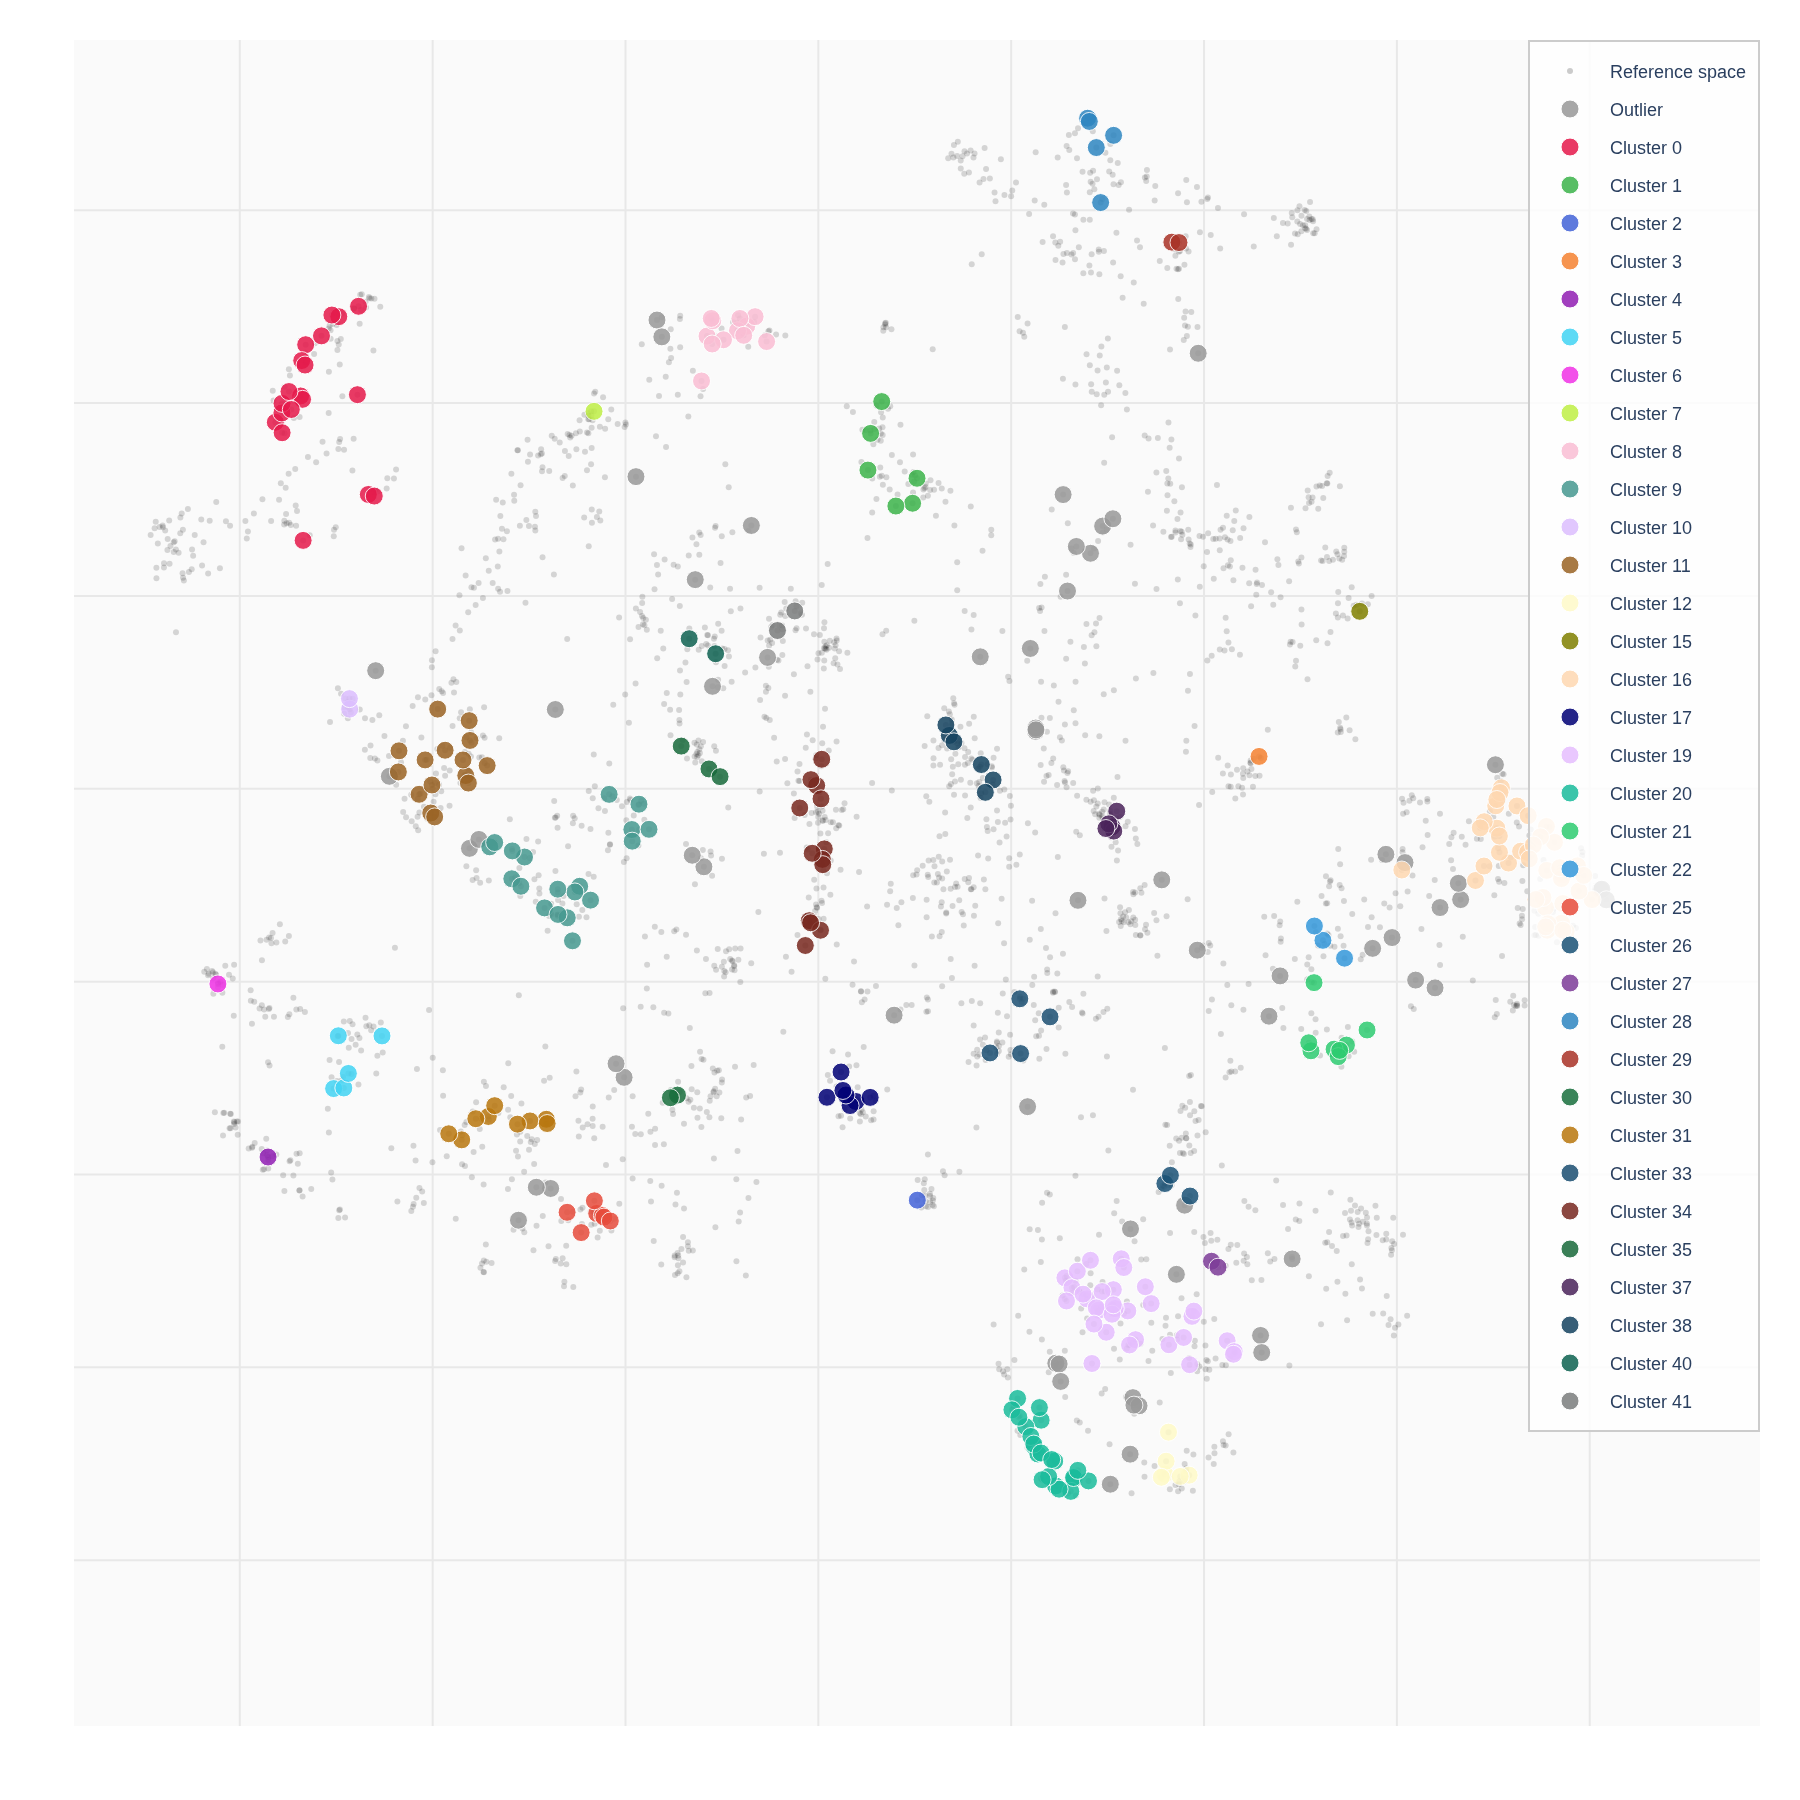
\includegraphics[width=0.85\linewidth]{figures/genomics-kidney-female-umap.png}\\
{\small\itshape Figure 1. GO Biological Process categories from the Kidney (Female) gene expression analysis projected onto a pre-computed UMAP embedding of GO BP terms. Points are colored by HDBSCAN semantic cluster.}
\end{center}
%% rlm:end item gene-sets::kidney-female-umap

%% rlm:begin item gene-sets::kidney-female-cluster
\begin{center}
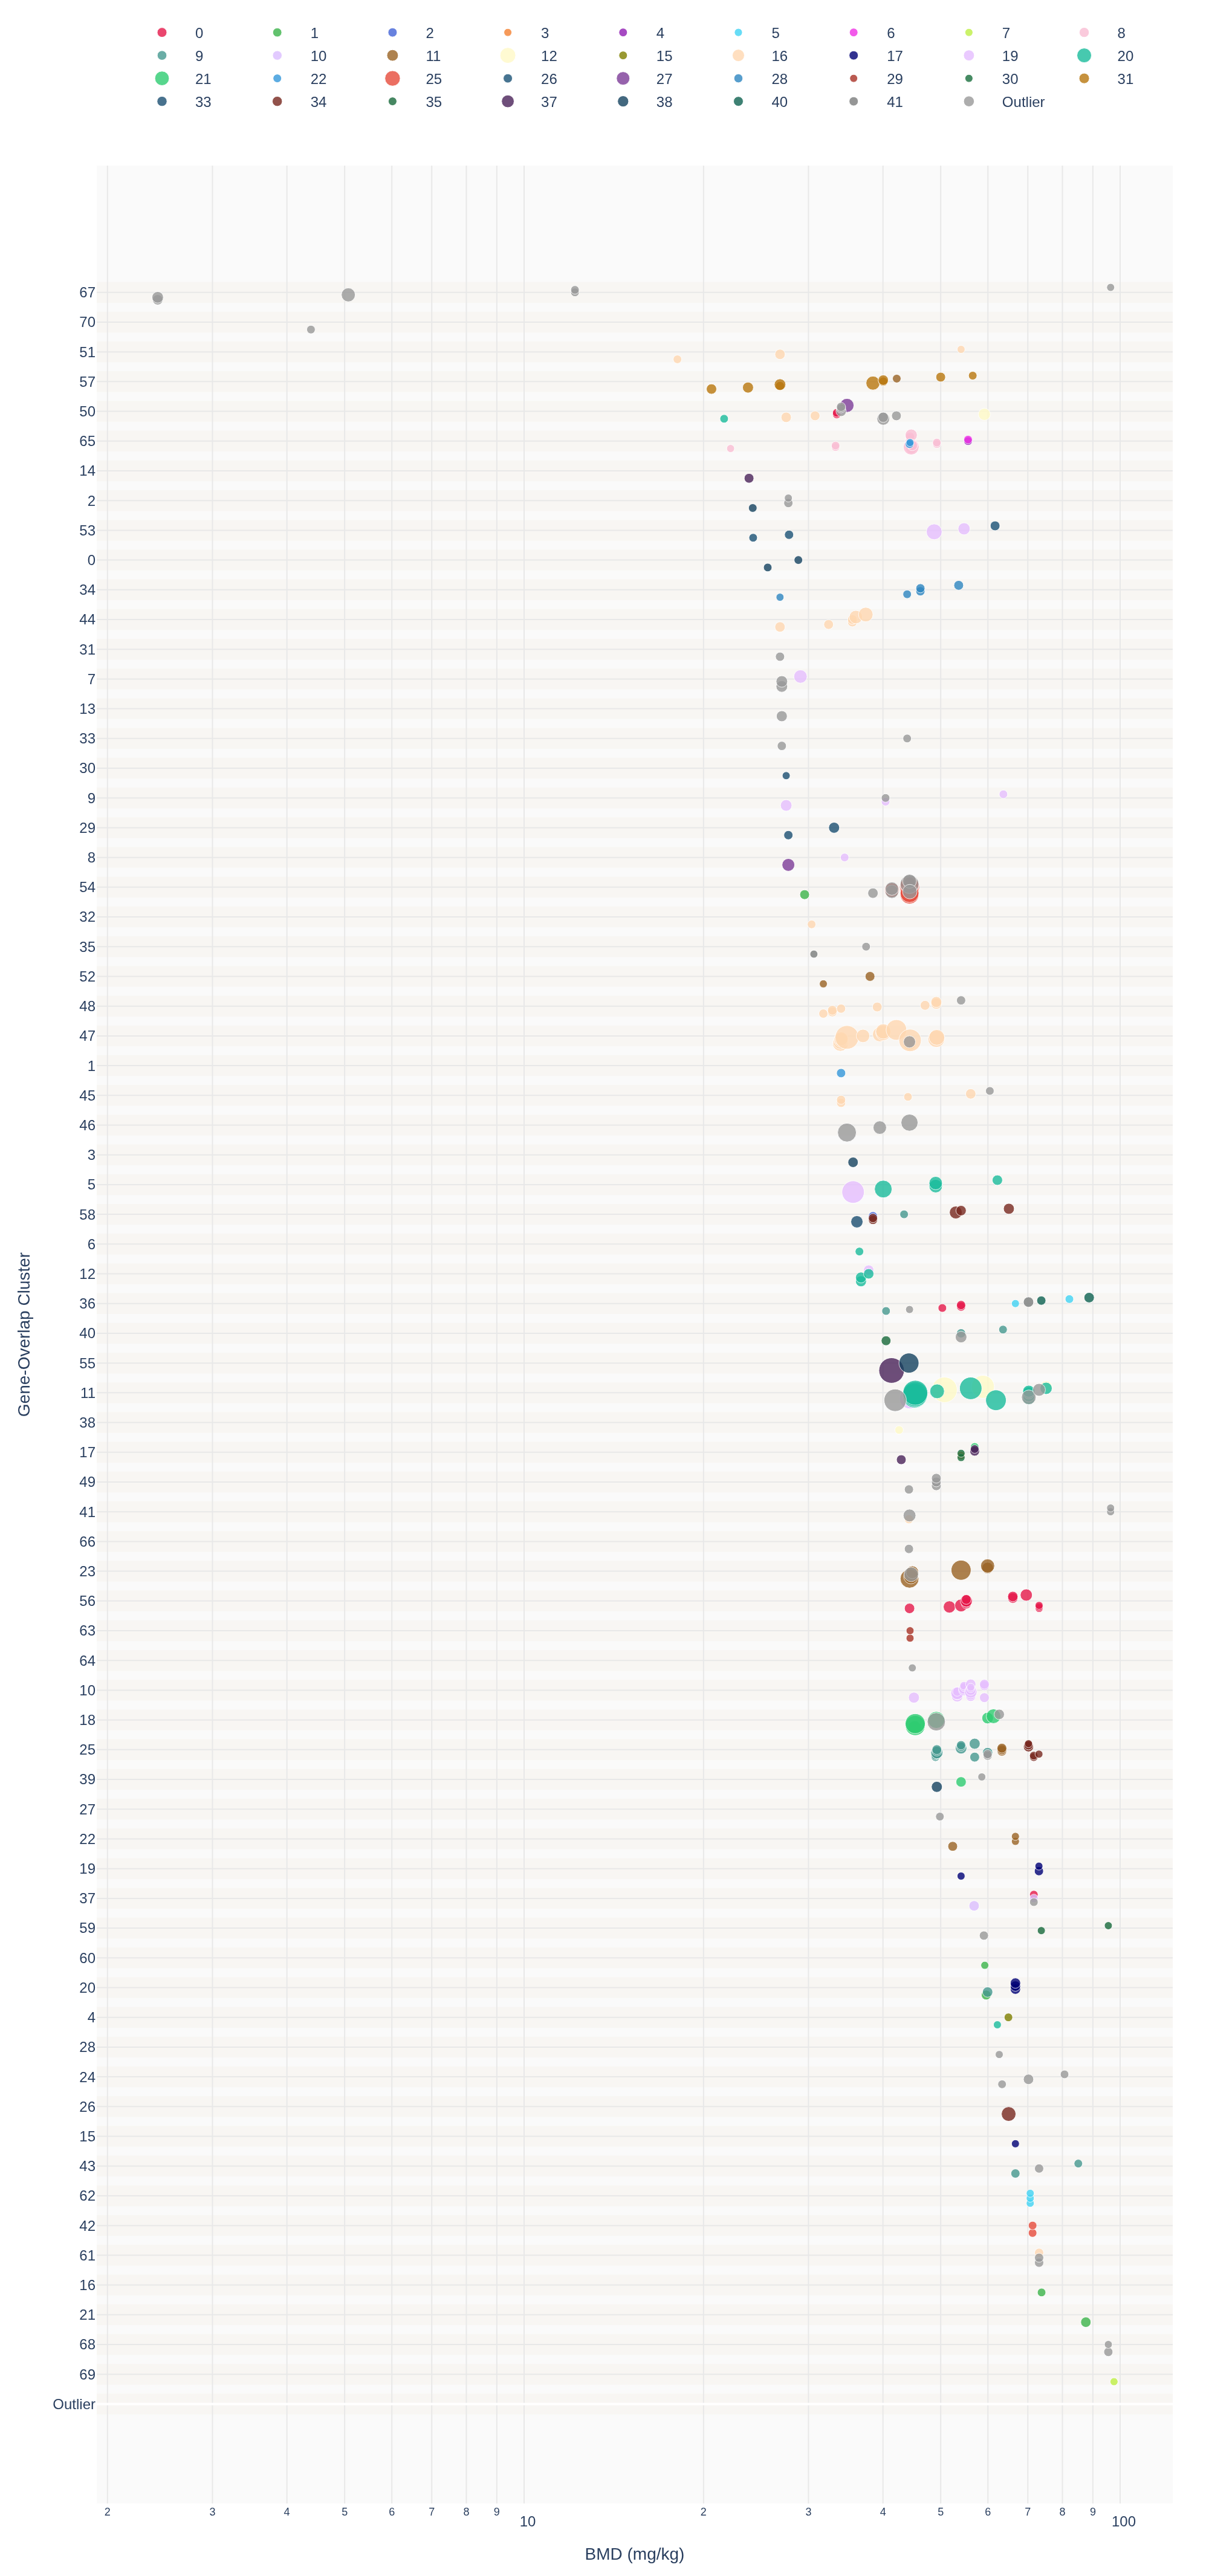
\includegraphics[width=0.85\linewidth]{figures/genomics-kidney-female-cluster.png}\\
{\small\itshape Figure 2. GO Biological Process categories from the Kidney (Female) analysis plotted by BMD value (x-axis, log scale) against hierarchical gene-overlap cluster assignment (y-axis). Marker size reflects the number of genes with BMD values in each category. Points are colored by UMAP semantic cluster (same palette as the semantic map above). Categories are clustered on the y-axis by Jaccard similarity of their gene sets.}
\end{center}
%% rlm:end item gene-sets::kidney-female-cluster

\subsubsection{Kidney, Male}

%% rlm:begin item gene-sets::kidney-male-narrative
Transcriptomic profiling of kidney tissue from male Sprague Dawley rats exposed to Perfluorohexanesulfonamide (PFHxSA) for 5 days identified 256 dose-responsive genes, of which 118 were upregulated and 138 were downregulated, indicating a predominantly suppressive transcriptional response. The most significantly enriched biological processes were centered on lipid and fatty acid metabolism, with GO terms for lipid metabolic process (66 genes, FDR=8.99e-36), fatty acid metabolic process (39 genes, FDR=2.04e-32), and fatty acid beta-oxidation (16 genes, FDR=2.52e-17) representing the dominant transcriptional signatures. The majority of genes contributing to fatty acid beta-oxidation and peroxisomal lipid catabolism—including ACOX1, ACAA1A, ACAA2, ACADM, ACADVL, EHHADH, and CPT2—were upregulated, consistent with activation of peroxisome proliferator-activated receptor alpha (PPAR-α) signaling, a well-established mechanism of action for perfluoroalkyl sulfonamide compounds. Corroborating this interpretation, KEGG pathway enrichment identified the PPAR signaling pathway (rno03320/hsa03320; ACOX1, PLIN2; FDR=1.70e-03) and metabolic pathways (rno01100/hsa01100; ACOX1, CYP2E1, GPX4; FDR=1.10e-03) as significantly enriched. Sterol and cholesterol biosynthetic processes were also prominently represented, with 12 genes in the sterol biosynthetic process GO term (FDR=3.65e-13) including HMGCR, HMGCS2, FDFT1, SQLE, and SREBF1, the majority of which were upregulated, suggesting coordinate induction of the mevalonate pathway. The xenobiotic metabolic process GO term (12 genes, FDR=2.50e-06) encompassed phase I and phase II enzymes including CYP2E1, UGT1A1, UGT2B15, UGT2B7, SULT1B1, and SULT1C3, indicating engagement of the xenobiotic detoxification machinery. The response to oxidative stress GO term (12 genes, FDR=5.41e-05) included GPX4, GPX2, and GSR, with a mixed directional pattern suggesting both adaptive antioxidant responses and potential perturbation of redox homeostasis.

BMD-ordered pathway analysis revealed that the earliest dose-responsive pathways, with median BMDs in the range of approximately 34–40 mg/kg/day, were the alcoholic liver disease pathway (rno04936/hsa04936; ACOX1, CYP2E1) and the PPAR signaling pathway (rno03320/hsa03320; ACOX1, PLIN2), followed closely by global metabolic pathways (rno01100/hsa01100). The arachidonic acid metabolism pathway (rno00590/hsa00590; CYP2E1, GPX4) exhibited a slightly higher median BMD of approximately 60.5 mg/kg/day, while the chemical carcinogenesis–reactive oxygen species pathway (hsa05208/rno05208; AHR, CYP2E1) showed the highest median BMD among enriched pathways at approximately 90.5 mg/kg/day, with a mixed directional response. This BMD ordering suggests that perturbation of fatty acid oxidation and PPAR-α-regulated lipid catabolism represents the most sensitive transcriptional response in the kidney, with oxidative stress and xenobiotic receptor-mediated responses occurring at higher doses. The overall pattern of upregulated peroxisomal and mitochondrial fatty acid oxidation genes, combined with induction of cholesterol biosynthesis and xenobiotic metabolism enzymes, is consistent with an adaptive hepatic-like metabolic reprogramming in the kidney, a response previously documented for PPAR-α-activating perfluoroalkyl substances. The bidirectional nature of the full gene set (118 up, 138 down), however, indicates that suppressive effects on additional biological processes—including cellular response to insulin stimulus (PCK1, INSIG1, SREBF1) and nutrient response pathways—co-occur with the inductive responses, suggesting a complex, potentially adverse disruption of renal metabolic homeostasis at higher doses.
%% rlm:end item gene-sets::kidney-male-narrative

%% rlm:begin item gene-sets::kidney-male-table
\adjustbox{max width=\linewidth}{%
\begin{tabular}{l l l r r r l}
\toprule
Rank & GO ID & Term & BMD & BMDL & Genes & Direction \\
\midrule
1 & GO:1902893 & regulation of miRNA transcription & 10.42 & 6.38 & 42 & up \\
2 & GO:2000628 & regulation of miRNA metabolic process & 10.42 & 6.38 & 45 & up \\
3 & GO:0010565 & regulation of cellular ketone metabolic process & 11.96 & 7.57 & 59 & up \\
4 & GO:0019217 & regulation of fatty acid metabolic process & 11.96 & 7.57 & 46 & up \\
5 & GO:0045598 & regulation of fat cell differentiation & 11.96 & 7.57 & 41 & up \\
6 & GO:0033273 & response to vitamin & 12.07 & 5.95 & 85 & up \\
7 & GO:0014910 & regulation of smooth muscle cell migration & 16.01 & 14.96 & 59 & up \\
8 & GO:0009743 & response to carbohydrate & 21.52 & 11.20 & 135 & up \\
9 & GO:0034284 & response to monosaccharide & 21.52 & 11.20 & 119 & up \\
10 & GO:0032869 & cellular response to insulin stimulus & 22.90 & 10.34 & 63 & up \\
11 & GO:0071375 & cellular response to peptide hormone stimulus & 24.68 & 13.00 & 123 & up \\
12 & GO:0002793 & positive regulation of peptide secretion & 25.64 & 9.19 & 52 & up \\
13 & GO:0032024 & positive regulation of insulin secretion & 25.64 & 9.19 & 41 & up \\
14 & GO:0051223 & regulation of protein transport & 25.64 & 8.20 & 153 & up \\
15 & GO:0070201 & regulation of establishment of protein localization & 25.64 & 8.20 & 178 & up \\
16 & GO:0090277 & positive regulation of peptide hormone secretion & 25.64 & 9.19 & 50 & up \\
17 & GO:0046434 & organophosphate catabolic process & 26.07 & 12.79 & 43 & up \\
18 & GO:1901136 & carbohydrate derivative catabolic process & 26.07 & 12.79 & 49 & up \\
19 & GO:0071383 & cellular response to steroid hormone stimulus & 26.12 & 14.63 & 62 & up \\
20 & GO:0071384 & cellular response to corticosteroid stimulus & 26.12 & 14.63 & 55 & up \\
\bottomrule
\end{tabular}
}
%% rlm:end item gene-sets::kidney-male-table

%% rlm:begin item gene-sets::kidney-male-umap
\begin{center}
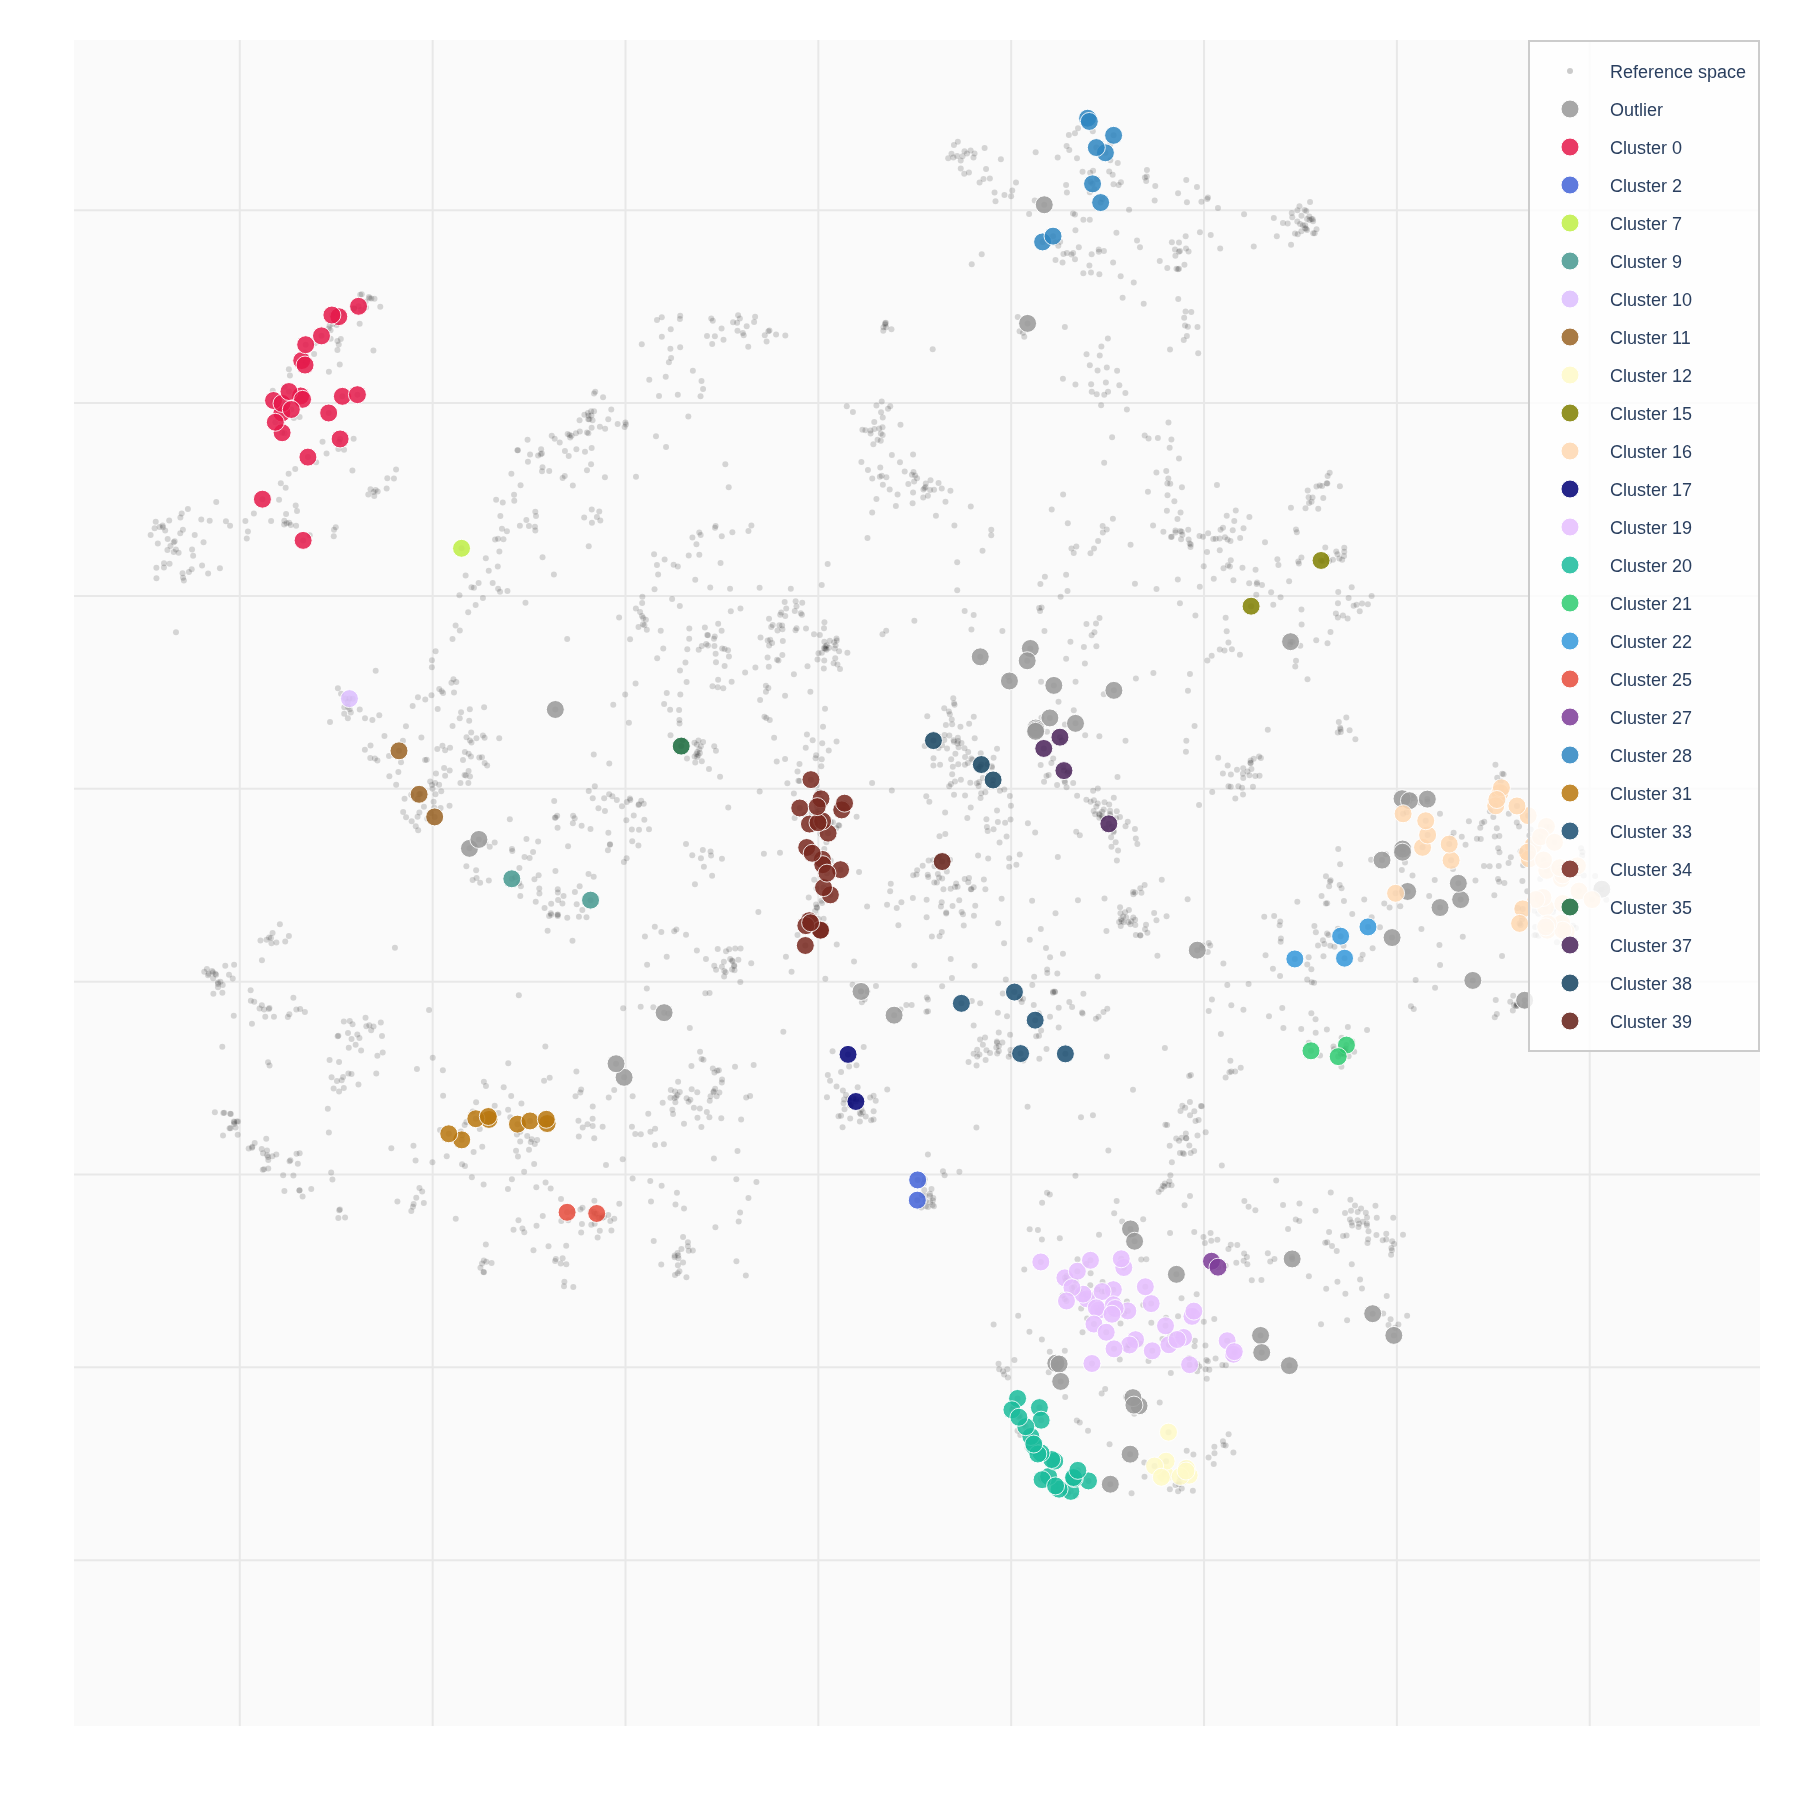
\includegraphics[width=0.85\linewidth]{figures/genomics-kidney-male-umap.png}\\
{\small\itshape Figure 3. GO Biological Process categories from the Kidney (Male) gene expression analysis projected onto a pre-computed UMAP embedding of GO BP terms. Points are colored by HDBSCAN semantic cluster.}
\end{center}
%% rlm:end item gene-sets::kidney-male-umap

%% rlm:begin item gene-sets::kidney-male-cluster
\begin{center}
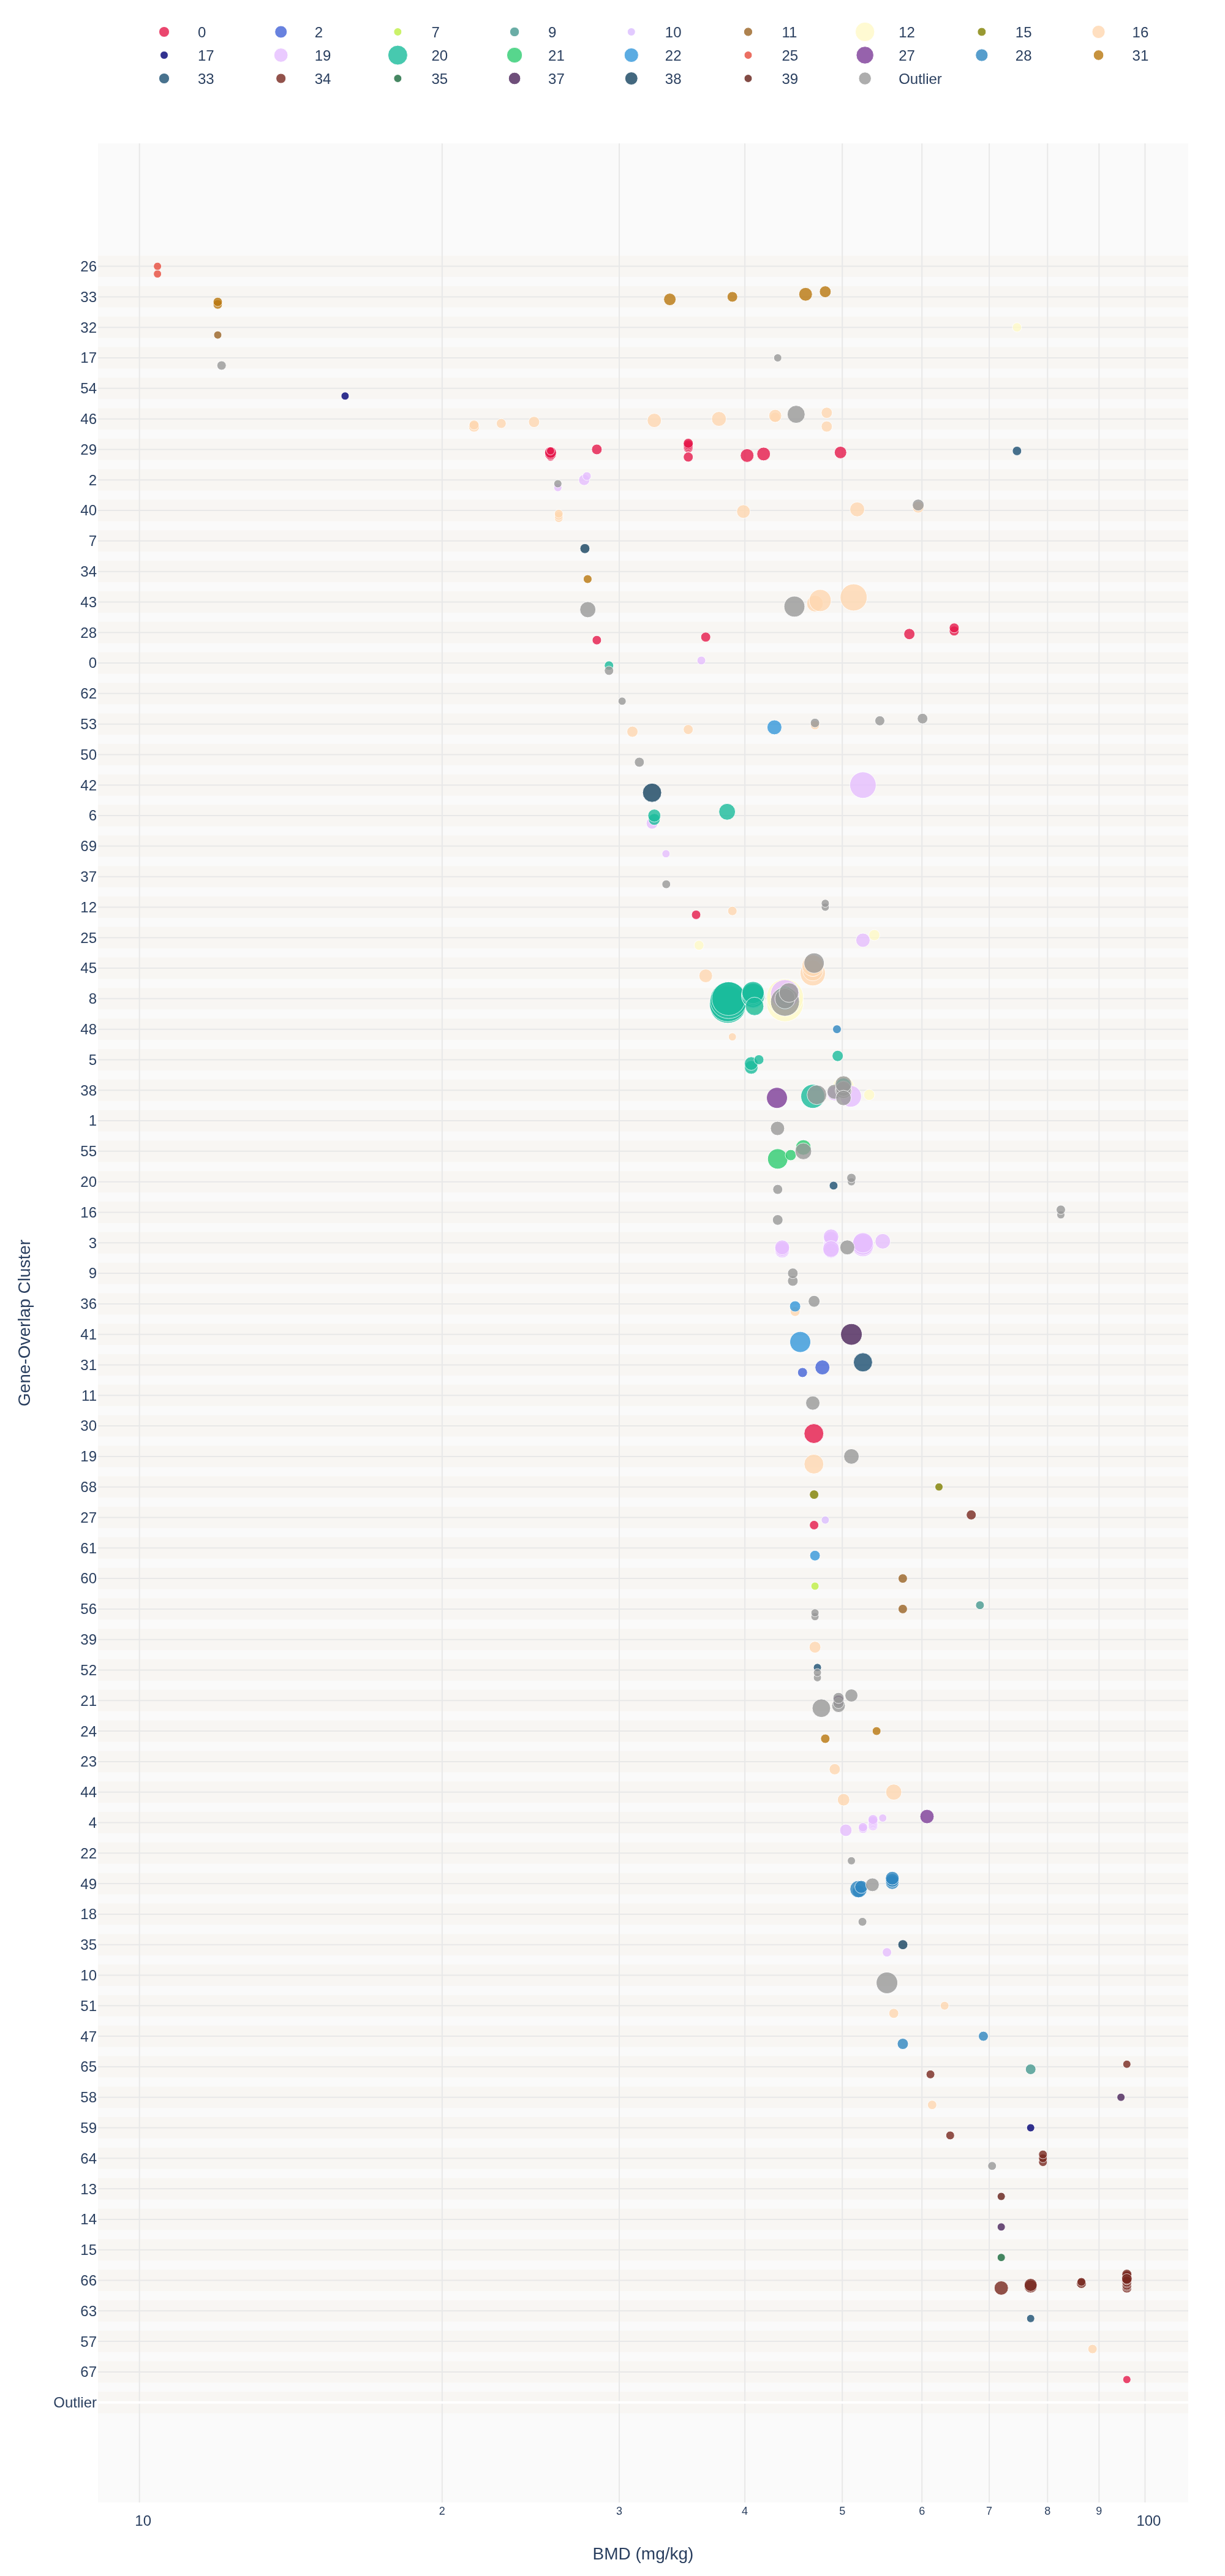
\includegraphics[width=0.85\linewidth]{figures/genomics-kidney-male-cluster.png}\\
{\small\itshape Figure 4. GO Biological Process categories from the Kidney (Male) analysis plotted by BMD value (x-axis, log scale) against hierarchical gene-overlap cluster assignment (y-axis). Marker size reflects the number of genes with BMD values in each category. Points are colored by UMAP semantic cluster (same palette as the semantic map above). Categories are clustered on the y-axis by Jaccard similarity of their gene sets.}
\end{center}
%% rlm:end item gene-sets::kidney-male-cluster

\subsubsection{Liver, Female}

%% rlm:begin item gene-sets::liver-female-narrative
Hepatic gene expression profiling in female Sprague Dawley rats following 5-day exposure to perfluorohexanesulfonamide (PFHxSA) identified 329 dose-responsive genes (256 upregulated, 73 downregulated; BMD range 0.814–366 mg/kg/day), indicating a predominantly transcriptional activation response. The most strongly enriched biological processes were fatty acid metabolic process (GO:0006631; 34 genes, FDR = 6.20×10⁻²²) and lipid metabolic process (GO:0006629; 54 genes, FDR = 5.30×10⁻¹⁹), with the large majority of constituent genes upregulated, a pattern consistent with peroxisome proliferator-activated receptor (PPAR) axis activation characteristic of perfluoroalkyl sulfonamide compounds. Fatty acid beta-oxidation (GO:0006635; 17 genes, FDR = 3.46×10⁻¹⁷) was similarly enriched, with upregulation of peroxisomal (ACOX1, ACOX2, EHHADH) and mitochondrial (ACADL, ACADM, ACADVL, CPT2, HADH, HADHB) oxidation genes, as well as acyl-CoA thioesterases (ACOT2, ACOT3, ACOT4, ACOT12) and fatty acid elongases (ELOVL5, ELOVL6), collectively indicating a broad induction of hepatic lipid catabolism and remodeling. Xenobiotic metabolic process (GO:0006805; 21 genes, FDR = 1.60×10⁻¹³) and response to xenobiotic stimulus (GO:0009410; 41 genes, FDR = 3.19×10⁻¹⁷) were also prominently enriched, driven by upregulation of multiple cytochrome P450 isoforms (CYP2B1, CYP2B2, CYP2B3, CYP2C11, CYP2D1, CYP2E1, CYP3A1, CYP3A2, CYP4A2) and phase II conjugation enzymes (GCLC, GSTA2, UGT1A1, UGT2B1), consistent with constitutive androstane receptor (CAR) and pregnane X receptor (PXR) co-activation. Response to oxidative stress (GO:0006979; 22 genes, FDR = 7.54×10⁻¹²) was enriched with predominantly upregulated antioxidant and proteasomal genes (SOD1, GCLC, GSR, TXNRD1, PRDX1, PRDX3, multiple PSMD subunits), suggesting an adaptive cellular defense response to oxidative burden. Additional enrichment of acute-phase response genes (GO:0006953; A2M, AHSG, F2, FGA, FN1, ORM1, SERPINA1; FDR = 1.80×10⁻⁶) and hemostasis-related genes (GO:0007599; FDR = 2.28×10⁻⁵) indicated broader hepatic stress signaling beyond lipid metabolism. Intracellular receptor signaling (GO:0030522; ESR1, NR1D2, NR1H3, NR1H4, NR1I3, PPARG, SREBF1; FDR = 5.15×10⁻⁵) and cholesterol homeostasis (GO:0042632; FDR = 9.41×10⁻⁵) were also enriched, with nuclear receptor genes predominantly upregulated, further supporting coordinate activation of lipid-sensing transcriptional programs.

Pathway enrichment analysis identified the PI3K–Akt signaling pathway (rno04151/hsa04151; FDR = 2.37×10⁻⁵) as the most significantly enriched KEGG pathway, represented by CDKN1A, FGF21, HGF, HSP90AA1, and MDM2, all predominantly upregulated. Thyroid cancer (rno05218/hsa05218; FDR = 6.06×10⁻⁵) and pathways in cancer (rno05200/hsa05200; FDR = 2.29×10⁻⁴) were enriched through the same gene set, reflecting the convergence of growth factor and cell cycle regulatory signaling rather than a cancer-specific response per se. Cellular senescence (hsa04218/rno04218; FDR = 1.99×10⁻³) was enriched via CDKN1A, MDM2, and SQSTM1, with genes predominantly upregulated, consistent with p53 pathway activation and stress-induced cell cycle arrest. Cell cycle (hsa04110/rno04110; FDR = 3.56×10⁻³) was represented by CDKN1A and MDM2 in a bidirectional pattern, suggesting mixed proliferative and antiproliferative signaling. Benchmark dose ordering of pathway-level responses revealed that metabolic pathways (rno01100; median BMD ≈ 49 mg/kg/day) were among the earliest to respond, followed by PI3K–Akt and cancer-related pathways (median BMD ≈ 54 mg/kg/day), cell cycle and senescence pathways (median BMD ≈ 58–76 mg/kg/day), and growth factor receptor signaling pathways including Ras, MAPK, and calcium signaling (median BMD ≈ 70 mg/kg/day). This BMD ordering suggests that perturbation of hepatic lipid and xenobiotic metabolism precedes activation of cell stress and proliferative signaling cascades, a sequence consistent with secondary genotoxic or cytotoxic mechanisms rather than direct DNA damage. The PPAR signaling pathway (rno03320/hsa03320; median BMD ≈ 55 mg/kg/day) was represented by predominantly upregulated genes, reinforcing PPAR-alpha as a primary molecular initiating event. Notably, hepatocellular carcinoma-related pathways (rno05205/hsa05205) showed a predominantly downregulated gene pattern (median BMD ≈ 76 mg/kg/day), which may reflect suppression of tumor suppressor or differentiation-associated signaling at higher doses.

Organ signature analysis predicted the strongest enrichment for liver-expressed genes (4.71-fold; 51+ genes), confirming the biological relevance of the hepatic transcriptional response. Enrichment was also observed for kidney, heart, muscle, and pancreas gene signatures, consistent with the known multi-organ distribution of perfluoroalkyl compounds and the broad expression of PPAR-regulated and oxidative stress genes across tissues. Enrichment of breast tissue (MCF-7 cell) signatures driven by ESR1 upregulation, and of immune system signatures driven by FGF21 and GDF15, suggests potential endocrine and systemic signaling perturbations secondary to hepatic metabolic reprogramming. The upregulation of mitophagy-associated genes (PINK1, TFAM, FIS1) contributed to enrichment of cardiomyocyte and pulmonary tissue signatures, indicating that mitochondrial quality control pathways were activated, potentially as an adaptive response to increased fatty acid oxidation flux and associated reactive oxygen species generation. Collectively, the transcriptional profile is consistent with a hepatic response dominated by PPAR-alpha–mediated lipid metabolic induction, coordinate xenobiotic enzyme induction via CAR/PXR, oxidative stress adaptation, and secondary activation of p53-associated cell cycle checkpoint and senescence pathways at higher doses, a pattern previously described for perfluoroalkyl sulfonyl compounds in rodent liver.
%% rlm:end item gene-sets::liver-female-narrative

%% rlm:begin item gene-sets::liver-female-table
\adjustbox{max width=\linewidth}{%
\begin{tabular}{l l l r r r l}
\toprule
Rank & GO ID & Term & BMD & BMDL & Genes & Direction \\
\midrule
1 & GO:0002698 & negative regulation of immune effector process & 9.62 & 8.19 & 45 & up \\
2 & GO:0002718 & regulation of cytokine production involved in immune response & 9.62 & 8.19 & 51 & down \\
3 & GO:0050764 & regulation of phagocytosis & 9.62 & 8.19 & 50 & down \\
4 & GO:0097191 & extrinsic apoptotic signaling pathway & 17.26 & 3.68 & 50 & up \\
5 & GO:0006650 & glycerophospholipid metabolic process & 17.41 & 7.01 & 53 & up \\
6 & GO:0045017 & glycerolipid biosynthetic process & 17.41 & 7.01 & 42 & up \\
7 & GO:1901136 & carbohydrate derivative catabolic process & 19.89 & 14.90 & 49 & up \\
8 & GO:0022408 & negative regulation of cell-cell adhesion & 20.30 & 7.54 & 64 & conflict \\
9 & GO:0032651 & regulation of interleukin-1 beta production & 21.73 & 8.19 & 41 & up \\
10 & GO:0050868 & negative regulation of T cell activation & 21.73 & 6.90 & 42 & up \\
11 & GO:0051250 & negative regulation of lymphocyte activation & 21.73 & 6.90 & 52 & up \\
12 & GO:1903038 & negative regulation of leukocyte cell-cell adhesion & 21.73 & 6.90 & 47 & up \\
13 & GO:0006720 & isoprenoid metabolic process & 22.16 & 13.77 & 41 & up \\
14 & GO:0032652 & regulation of interleukin-1 production & 22.19 & 6.90 & 48 & up \\
15 & GO:0032760 & positive regulation of tumor necrosis factor production & 22.19 & 8.09 & 54 & up \\
16 & GO:1903557 & positive regulation of tumor necrosis factor superfamily cytokine production & 22.19 & 8.09 & 55 & up \\
17 & GO:0006805 & xenobiotic metabolic process & 22.53 & 10.59 & 59 & up \\
18 & GO:0046486 & glycerolipid metabolic process & 22.58 & 10.58 & 75 & up \\
19 & GO:0032680 & regulation of tumor necrosis factor production & 22.66 & 5.68 & 76 & up \\
20 & GO:1903555 & regulation of tumor necrosis factor superfamily cytokine production & 22.66 & 5.68 & 77 & up \\
\bottomrule
\end{tabular}
}
%% rlm:end item gene-sets::liver-female-table

%% rlm:begin item gene-sets::liver-female-umap
\begin{center}
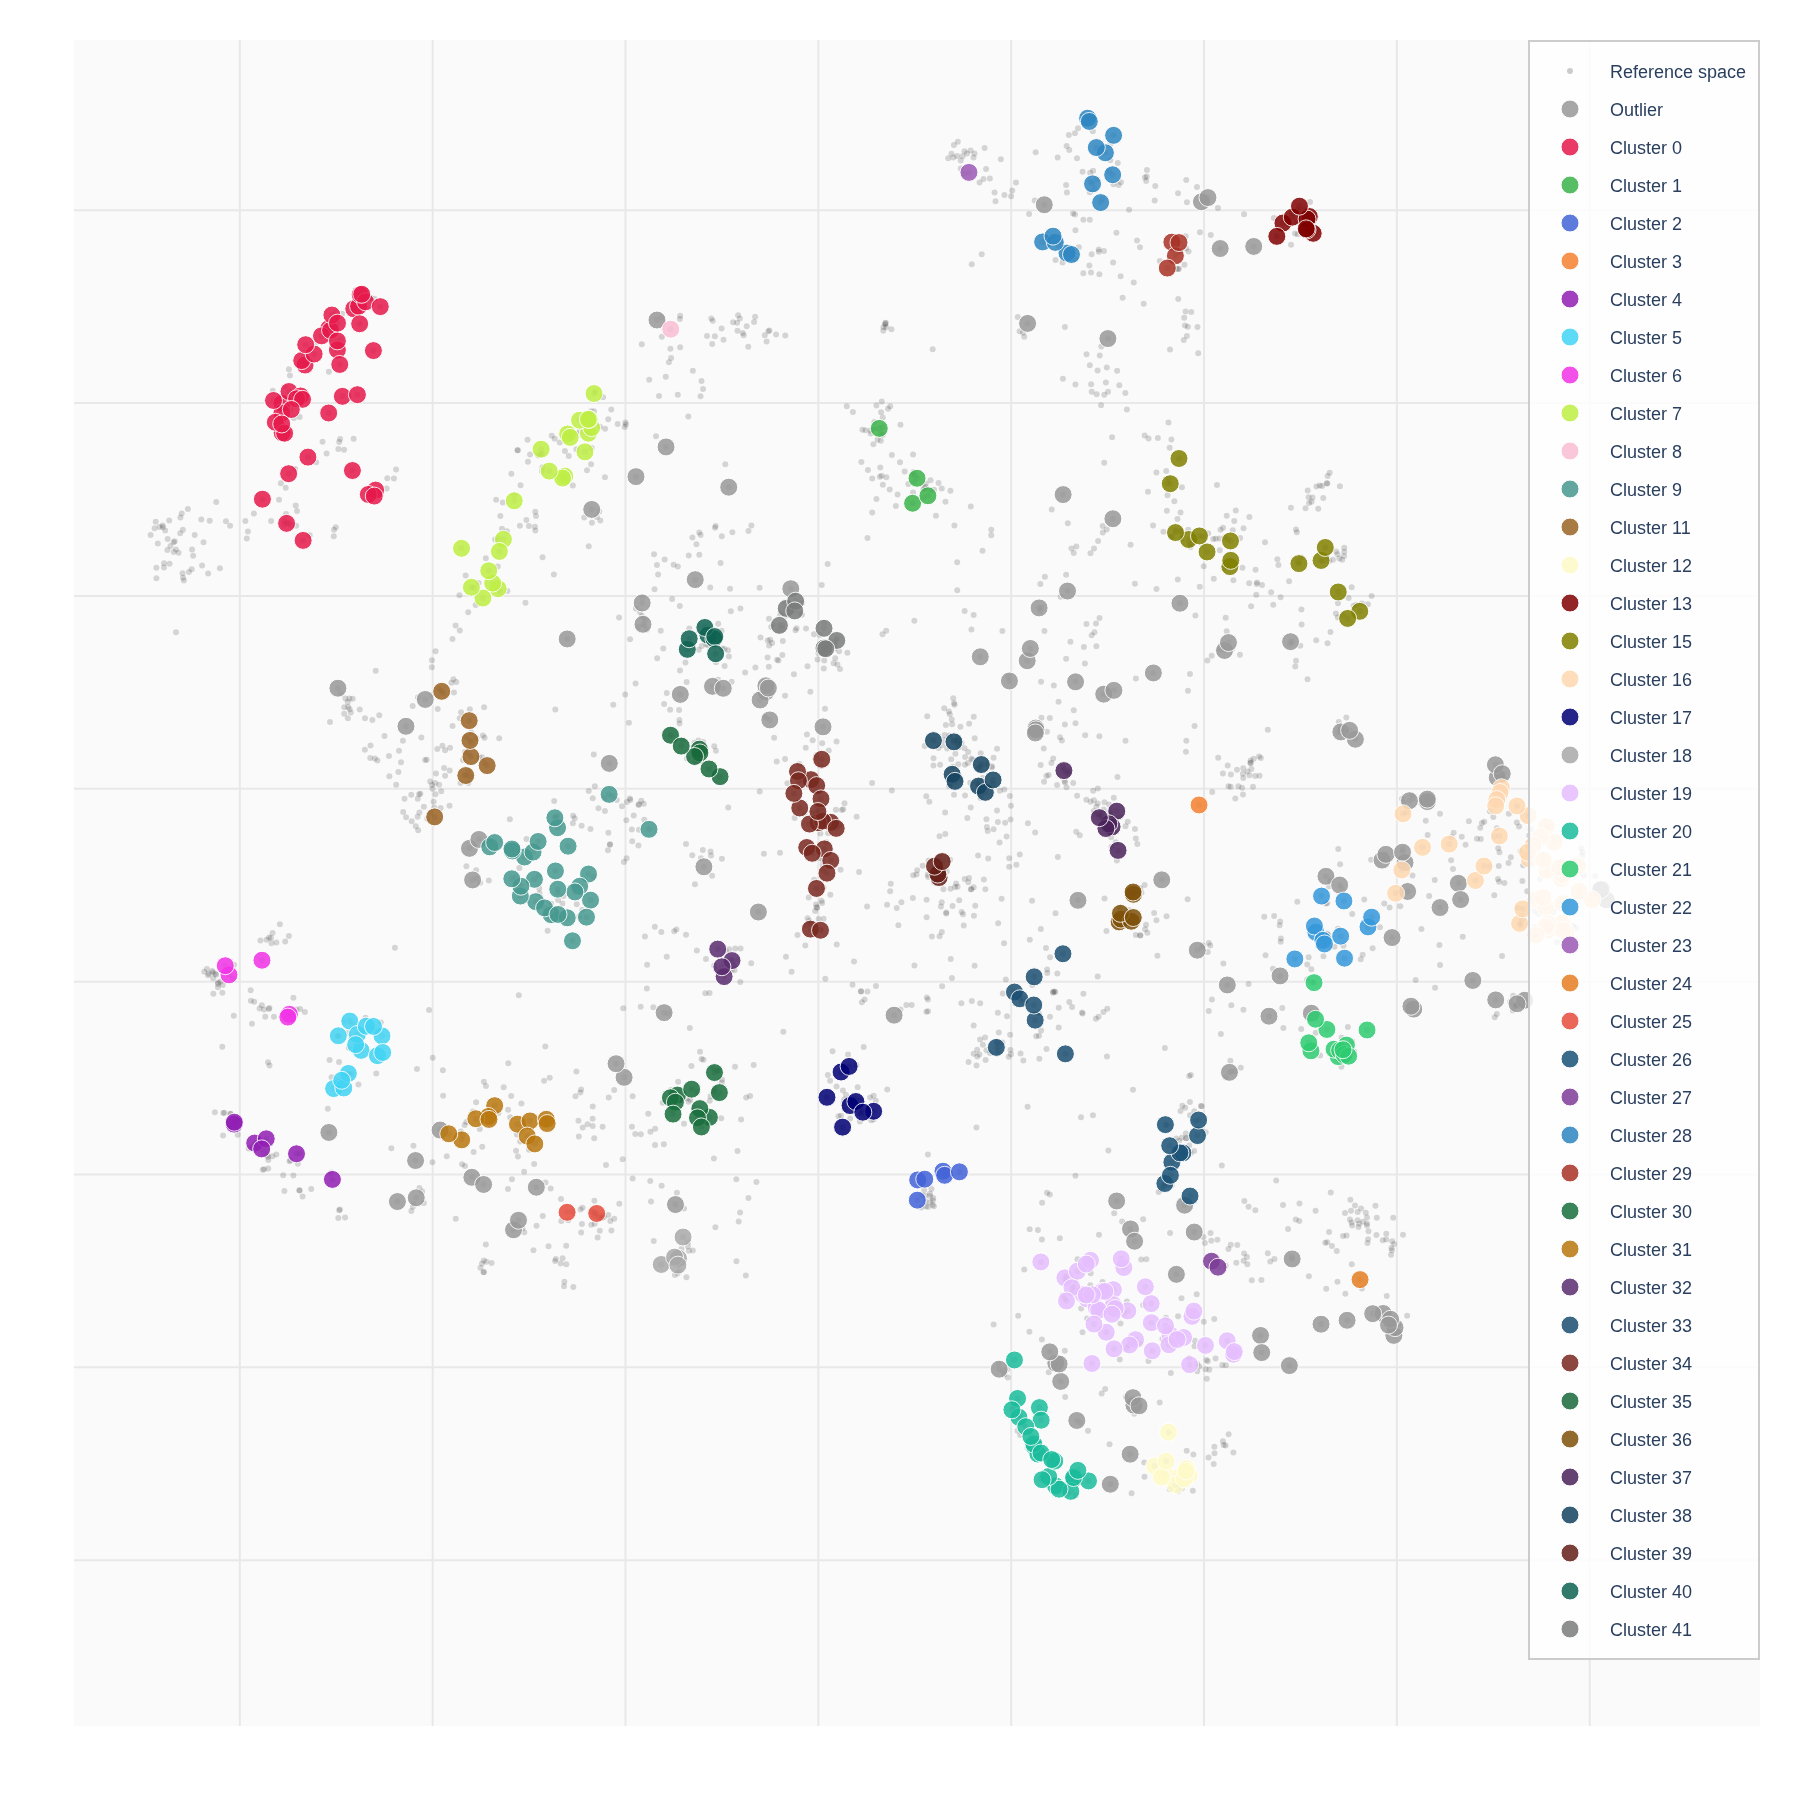
\includegraphics[width=0.85\linewidth]{figures/genomics-liver-female-umap.png}\\
{\small\itshape Figure 5. GO Biological Process categories from the Liver (Female) gene expression analysis projected onto a pre-computed UMAP embedding of GO BP terms. Points are colored by HDBSCAN semantic cluster.}
\end{center}
%% rlm:end item gene-sets::liver-female-umap

%% rlm:begin item gene-sets::liver-female-cluster
\begin{center}
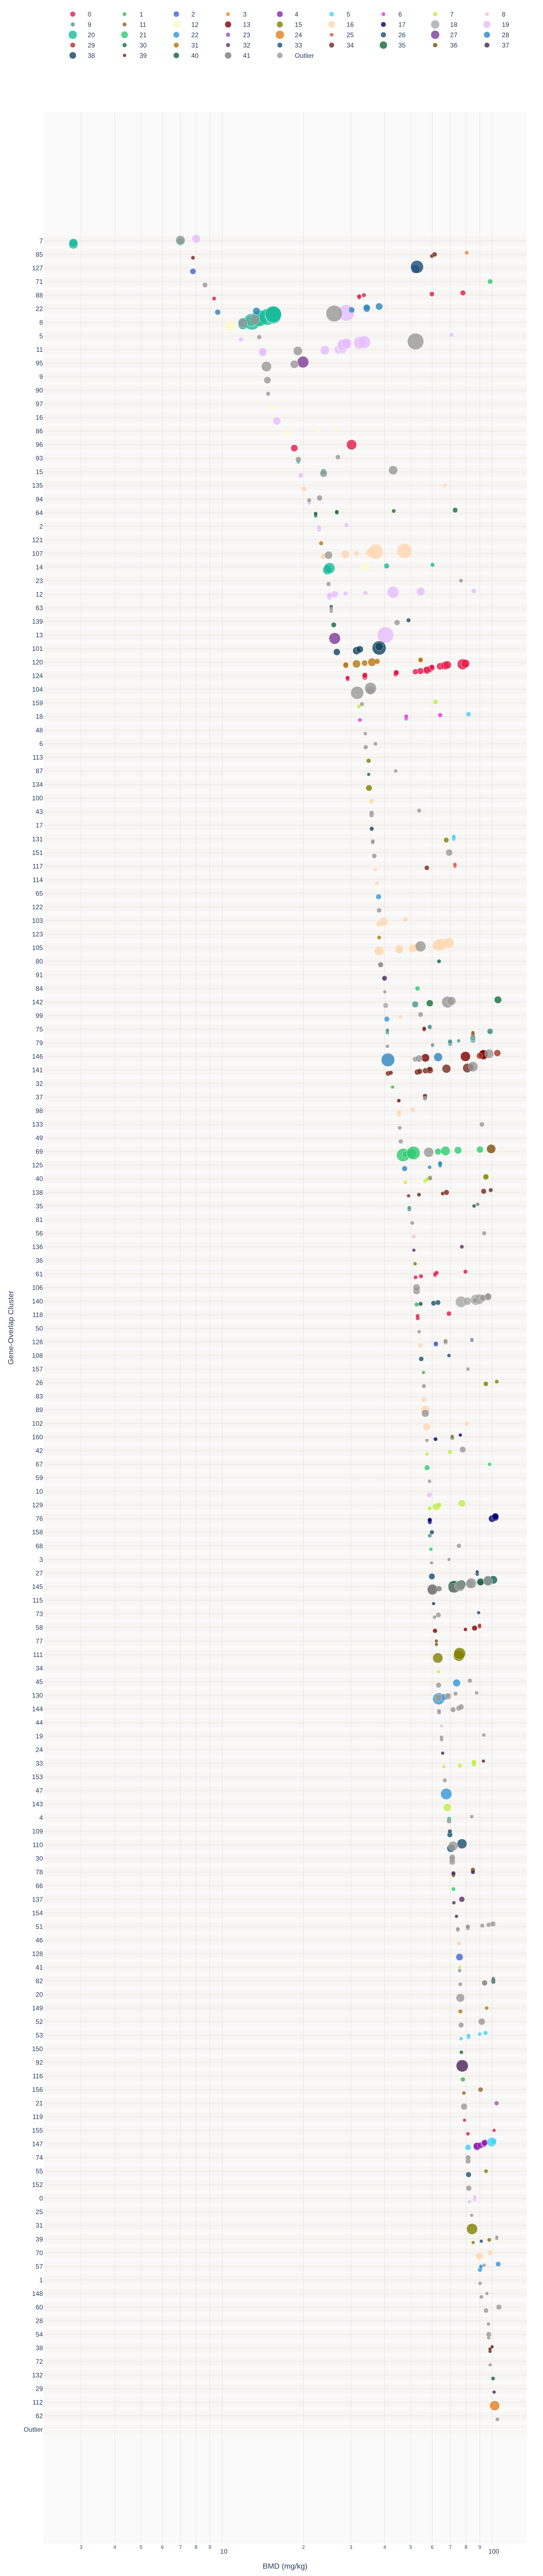
\includegraphics[width=0.85\linewidth]{figures/genomics-liver-female-cluster.png}\\
{\small\itshape Figure 6. GO Biological Process categories from the Liver (Female) analysis plotted by BMD value (x-axis, log scale) against hierarchical gene-overlap cluster assignment (y-axis). Marker size reflects the number of genes with BMD values in each category. Points are colored by UMAP semantic cluster (same palette as the semantic map above). Categories are clustered on the y-axis by Jaccard similarity of their gene sets.}
\end{center}
%% rlm:end item gene-sets::liver-female-cluster

\subsubsection{Liver, Male}

%% rlm:begin item gene-sets::liver-male-narrative
Hepatic gene expression profiling in male Sprague-Dawley rats following 5-day exposure to perfluorohexanesulfonamide (PFHxSA) identified 461 dose-responsive genes (259 upregulated, 202 downregulated) with benchmark doses (BMDs) spanning approximately 0.06 to 379 mg/kg/day. The most significantly enriched biological processes were response to xenobiotic stimulus (GO:0009410; 68 genes, FDR = 6.66×10⁻³⁴) and lipid metabolic process (GO:0006629; 81 genes, FDR = 1.12×10⁻³¹), followed by fatty acid metabolic process (GO:0006631; 39 genes, FDR = 9.63×10⁻²³) and fatty acid beta-oxidation (GO:0006635; 19 genes, FDR = 1.40×10⁻¹⁷). The predominant upregulation of genes within the metabolic pathway enrichment cluster—including ACOX1, EHHADH, ACAA1A, ACADM, and ACADVL—is consistent with peroxisome proliferator-activated receptor alpha (PPARα) activation, a well-established mechanism of action for perfluoroalkyl sulfonamide compounds. This interpretation is further supported by significant enrichment of the PPAR signaling pathway (path:rno03320/hsa03320; ACOX1, CYP7A1, PLIN2; FDR = 6.10×10⁻⁴) and the non-alcoholic fatty liver disease pathway (path:rno04936/hsa04936; ACOX1, CYP2E1, FOXO3, PPARGC1A; FDR = 6.51×10⁻⁴), with the majority of constituent genes upregulated, reflecting an adaptive transcriptional response to increased fatty acid flux. Concurrent enrichment of response to oxidative stress (GO:0006979; 27 genes, FDR = 2.51×10⁻¹³) and xenobiotic metabolic process (GO:0006805; 27 genes, FDR = 8.81×10⁻¹⁷) further indicates that PFHxSA exposure elicited a coordinated hepatic detoxification and antioxidant response, with upregulation of NFE2L2, HMOX1, GPX4, SOD1, SOD2, and TXNRD1 consistent with Nrf2 pathway activation. The acute-phase response (GO:0006953; 15 genes, FDR = 3.49×10⁻¹²) was also significantly enriched, with genes such as STAT3, HP, ORM1, and SERPINA1 represented, suggesting a hepatic inflammatory component to the response.

BMD-ordered pathway analysis revealed a structured, dose-dependent progression of transcriptional perturbations. The lowest-BMD responses (median BMD \textasciitilde{}3.7 mg/kg/day) involved downregulation of genes in the GnRH secretion and viral infection pathways (path:hsa04928, path:hsa05166), suggesting that neuroendocrine and immune-related transcriptional changes may represent early, sensitive endpoints. Pathways related to FoxO signaling (path:hsa04068), PI3K-Akt signaling (path:hsa04151), and cancer-associated signaling (path:hsa05223, path:hsa05225) exhibited median BMDs in the range of approximately 8–10 mg/kg/day, predominantly in the downward direction, indicating suppression of proliferative and survival signaling at moderate doses. The metabolic pathways most strongly associated with PPARα activation—including PPAR signaling (path:rno03320) and metabolic pathways (path:rno01100)—displayed median BMDs of approximately 28 mg/kg/day with predominantly upregulated gene members, consistent with an adaptive lipid-catabolic response occurring at higher doses. Pathways involving HIF-1 signaling (path:hsa04066), chemical carcinogenesis (path:hsa05208), and fluid shear stress (path:hsa05418) showed median BMDs in the range of 21–31 mg/kg/day with predominantly downregulated genes, suggesting that perturbation of stress-responsive and vascular signaling pathways occurs at intermediate-to-high exposure levels. Taken together, the BMD ordering indicates that the earliest transcriptional responses to PFHxSA involve downregulation of signaling pathways governing cell survival and endocrine function, followed at higher doses by induction of lipid metabolism and antioxidant defense programs.

Organ signature analysis indicated that the transcriptional profile observed in rat liver was most strongly enriched relative to liver-specific gene expression databases (4.35-fold enrichment; 66+ genes), consistent with the hepatic tissue of origin. Significant cross-tissue enrichment was also observed for kidney (3.67-fold), heart (3.56-fold), and multiple neural and immune tissues, driven primarily by the broad expression of consensus stress-response genes including NFE2L2, HMOX1, GPX4, STAT3, and CDKN1A. The high enrichment scores observed for nasal fibroblasts, blood-brain barrier, and substantia nigra tissues (19–48-fold) reflect the known multi-tissue activity of Nrf2-target genes rather than primary target organ specificity. The enrichment of skeletal muscle and inguinal adipose tissue signatures (32-fold; PPARGC1A, SIRT3) is consistent with the known role of PGC-1α in mitochondrial biogenesis and energy metabolism, suggesting that PFHxSA may perturb mitochondrial homeostasis in addition to lipid catabolism. The overall pattern of pathway enrichment, BMD distribution, and organ signature is consistent with a hepatic response dominated by PPARα-mediated lipid metabolic reprogramming and Nrf2-driven oxidative stress adaptation, with secondary perturbation of cell cycle regulation, acute-phase signaling, and growth factor pathways at higher doses.
%% rlm:end item gene-sets::liver-male-narrative

%% rlm:begin item gene-sets::liver-male-table
\adjustbox{max width=\linewidth}{%
\begin{tabular}{l l l r r r l}
\toprule
Rank & GO ID & Term & BMD & BMDL & Genes & Direction \\
\midrule
1 & GO:0032368 & regulation of lipid transport & 3.84 & 2.77 & 45 & down \\
2 & GO:0030111 & regulation of Wnt signaling pathway & 4.91 & 1.48 & 65 & down \\
3 & GO:0008203 & cholesterol metabolic process & 6.42 & 5.11 & 54 & down \\
4 & GO:0016125 & sterol metabolic process & 6.42 & 5.11 & 56 & down \\
5 & GO:0048568 & embryonic organ development & 7.82 & 1.69 & 47 & down \\
6 & GO:0055088 & lipid homeostasis & 7.84 & 3.84 & 58 & down \\
7 & GO:0032526 & response to retinoic acid & 8.76 & 5.20 & 51 & up \\
8 & GO:0043525 & positive regulation of neuron apoptotic process & 8.79 & 2.63 & 45 & down \\
9 & GO:0045582 & positive regulation of T cell differentiation & 8.79 & 2.63 & 40 & down \\
10 & GO:0045621 & positive regulation of lymphocyte differentiation & 8.79 & 2.63 & 43 & down \\
11 & GO:0045637 & regulation of myeloid cell differentiation & 8.79 & 2.63 & 73 & down \\
12 & GO:0060828 & regulation of canonical Wnt signaling pathway & 8.79 & 2.63 & 50 & down \\
13 & GO:0071229 & cellular response to acid chemical & 9.78 & 2.29 & 54 & down \\
14 & GO:0010720 & positive regulation of cell development & 9.93 & 6.73 & 145 & down \\
15 & GO:0045580 & regulation of T cell differentiation & 9.93 & 6.73 & 54 & conflict \\
16 & GO:0045619 & regulation of lymphocyte differentiation & 9.93 & 6.73 & 60 & conflict \\
17 & GO:0051251 & positive regulation of lymphocyte activation & 9.93 & 6.73 & 102 & conflict \\
18 & GO:1902107 & positive regulation of leukocyte differentiation & 9.93 & 6.73 & 64 & down \\
19 & GO:1903708 & positive regulation of hemopoiesis & 9.93 & 6.73 & 64 & down \\
20 & GO:0002696 & positive regulation of leukocyte activation & 11.07 & 10.82 & 109 & conflict \\
\bottomrule
\end{tabular}
}
%% rlm:end item gene-sets::liver-male-table

%% rlm:begin item gene-sets::liver-male-umap
\begin{center}
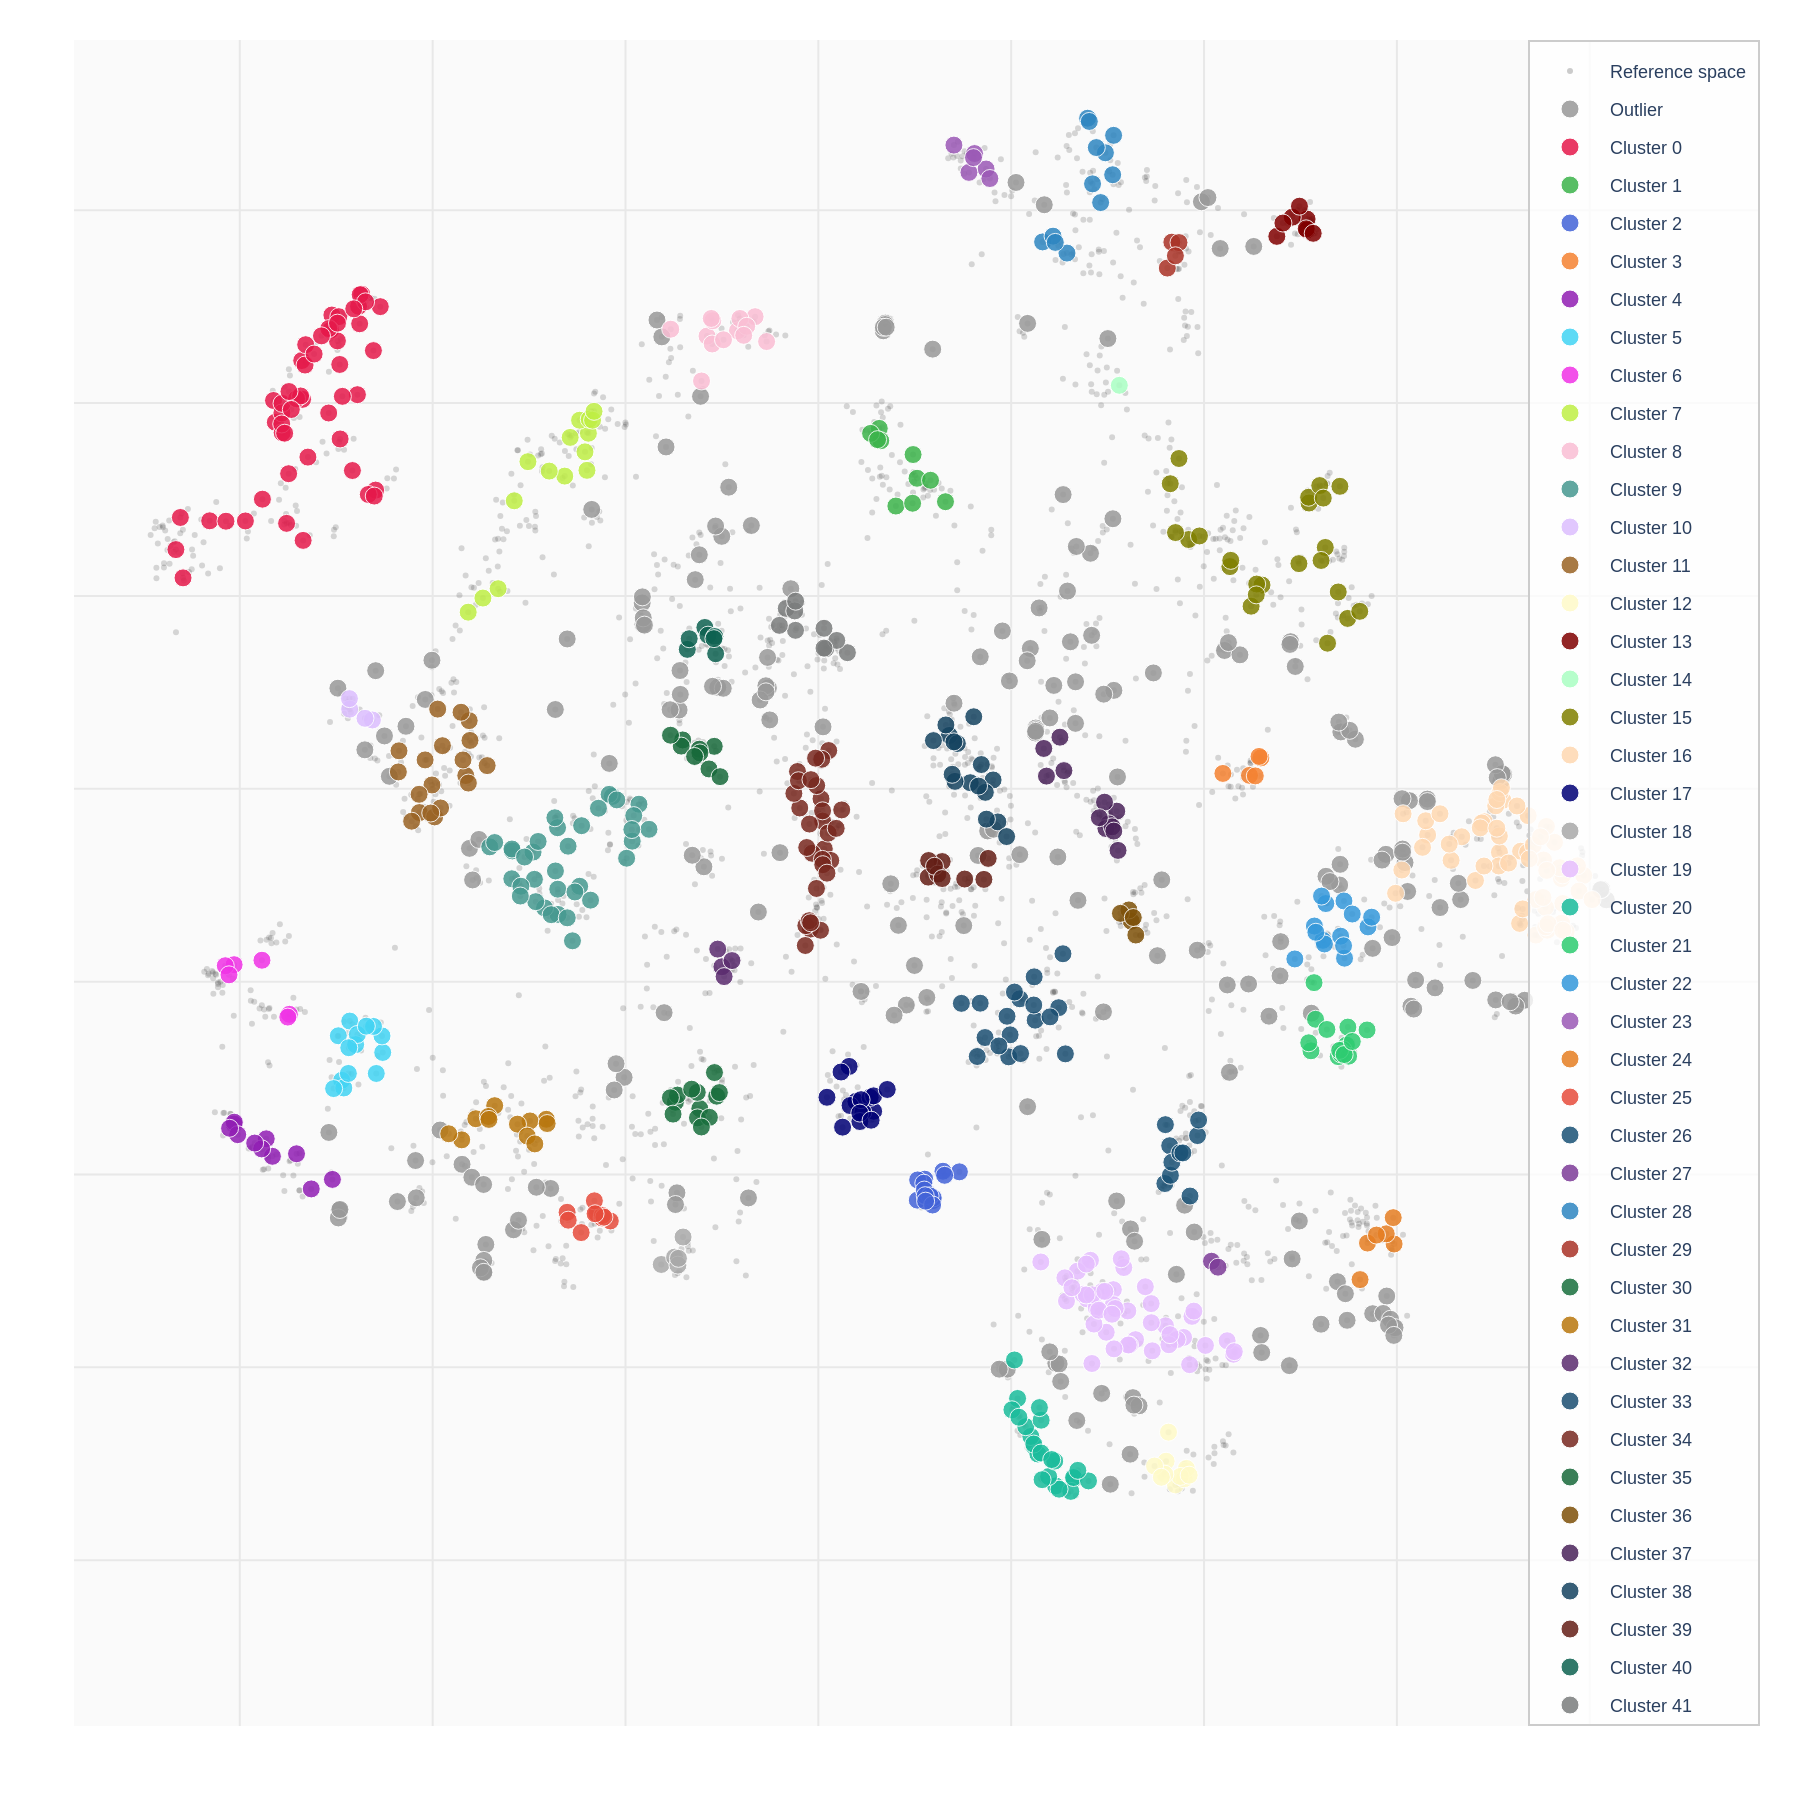
\includegraphics[width=0.85\linewidth]{figures/genomics-liver-male-umap.png}\\
{\small\itshape Figure 7. GO Biological Process categories from the Liver (Male) gene expression analysis projected onto a pre-computed UMAP embedding of GO BP terms. Points are colored by HDBSCAN semantic cluster.}
\end{center}
%% rlm:end item gene-sets::liver-male-umap

%% rlm:begin item gene-sets::liver-male-cluster
\begin{center}

\includegraphics[width=0.85\linewidth]{figures/genomics-liver-male-cluster.png}\\
{\small\itshape Figure 8. GO Biological Process categories from the Liver (Male) analysis plotted by BMD value (x-axis, log scale) against hierarchical gene-overlap cluster assignment (y-axis). Marker size reflects the number of genes with BMD values in each category. Points are colored by UMAP semantic cluster (same palette as the semantic map above). Categories are clustered on the y-axis by Jaccard similarity of their gene sets.}
\end{center}
%% rlm:end item gene-sets::liver-male-cluster
%% rlm:end node gene-sets

%% rlm:begin node gene-bmd
\subsection{Gene Benchmark Dose Analysis}

\subsubsection{Kidney, Female}

%% rlm:begin item gene-bmd::kidney-female-narrative
Among individual genes, CDKN1A (p21/WAF1/CIP1) emerged as one of the most sensitive and biologically informative responders, with a BMD of approximately 44.4 mg/kg/day and upregulated expression. CDKN1A is a well-established marker of genotoxic and cytostatic stress, and its induction in the kidney is consistent with cell cycle arrest at the G1/S checkpoint. The literature support for CDKN1A as a toxicogenomic marker is extensive, with 52 supporting publications identifying this gene across a broad range of tissues and chemical exposures; notably, CDKN1A has been validated as one of four functional genotoxic marker genes capable of distinguishing genotoxic from non-genotoxic hepatocarcinogens in rat liver, lending high confidence to its interpretation as a stress-responsive indicator in the present renal context. HIF1A and VEGFA, both upregulated with BMDs in the range of 118 mg/kg/day, were identified as consensus genes supported by 44 and 45 publications, respectively, and their co-enrichment in renal cell carcinoma and HIF-1 signaling pathways is mechanistically coherent. HIF1A upregulation in the kidney is consistent with transcriptomic responses reported for ochratoxin A and cobalt, where AhR-Smad2/3-HIF-1α signaling mediates nephrotoxicity, and VEGFA induction has been linked to modulation of renal vascular permeability and angiogenic signaling under chemical stress. SQSTM1 (p62), upregulated with a BMD of approximately 153 mg/kg/day, is a multifunctional scaffold protein involved in autophagy receptor signaling and NRF2 pathway activation; its co-enrichment with HIF1A in autophagy and mitophagy pathways, and its literature support across 23 publications in metabolic and neurodegenerative contexts, supports interpretation of its induction as part of a coordinated mitochondrial stress response.
%% rlm:end item gene-bmd::kidney-female-narrative

%% rlm:begin item gene-bmd::kidney-female-table
\adjustbox{max width=\linewidth}{%
\begin{tabular}{l l r r l r}
\toprule
Rank & Gene & BMD & BMDL & Direction & Fold Change \\
\midrule
1 & TNNI1 & 0.39 & 0.06 & up & 1.39 \\
2 & CDKN3 & 1.10 & 0.33 & up & 1.81 \\
3 & CKAP2 & 1.38 & 0.32 & up & 1.86 \\
4 & CDCA3 & 1.41 & 0.42 & up & 2.01 \\
5 & RACGAP1 & 2.08 & 0.24 & up & 1.47 \\
6 & CCNB2 & 2.14 & 0.48 & up & 1.70 \\
7 & KIF18B & 2.43 & 0.54 & up & 1.64 \\
8 & CEBPD & 2.66 & 0.26 & up & 1.31 \\
9 & UBE2T & 3.37 & 0.72 & up & 1.93 \\
10 & CYP2C24 & 3.42 & 0.71 & down & -1.98 \\
11 & SPC24 & 3.71 & 0.92 & up & 1.56 \\
12 & CYP24A1 & 4.10 & 0.76 & up & 2.21 \\
13 & KNTC1 & 5.07 & 1.83 & up & 1.71 \\
14 & CYR61 & 5.30 & 0.63 & up & 1.39 \\
15 & SLC10A1 & 6.77 & 1.77 & down & -2.18 \\
16 & PCK1 & 7.69 & 6.47 & up & 2.19 \\
17 & SREBF1 & 9.29 & 2.97 & up & 2.77 \\
18 & SULT1C2 & 14.93 & 12.16 & down & -1.81 \\
19 & LOC100911814 & 17.24 & 0.76 & up & 1.60 \\
20 & GSTA2 & 19.85 & 4.55 & up & 1.45 \\
\bottomrule
\end{tabular}
}
%% rlm:end item gene-bmd::kidney-female-table

\subsubsection{Kidney, Male}

%% rlm:begin item gene-bmd::kidney-male-narrative
Among the individual dose-responsive genes, GPX4 emerged as a high-confidence sentinel gene supported by an extensive literature base (156 papers), with broad organ-level enrichment spanning kidney, liver, testes, and numerous other tissues. GPX4 encodes glutathione peroxidase 4, a critical regulator of ferroptosis through its role in reducing phospholipid hydroperoxides, and its dose-responsive alteration in the kidney is consistent with PFAS-associated oxidative lipid stress. The co-regulation of GPX4 with FASN—whose knockdown has been shown to promote GPX4 degradation and ferroptosis—and with SQSTM1, a mediator of selective autophagy implicated in the GPX4/SQSTM1 ferroptotic axis in gastric cancer models, raises the possibility that PFHxSA exposure perturbs ferroptosis-regulatory networks in the kidney. AHR, a well-established xenobiotic receptor and transcriptional regulator, was identified as a dose-responsive gene with strong literature support (35 papers) and enrichment in kidney, liver, and male reproductive organ signatures; its co-enrichment with CYP2E1 in the chemical carcinogenesis pathway at a median BMD of approximately 90.5 mg/kg/day is consistent with AHR-mediated induction of oxidative metabolism at higher exposure levels. CYP11A1, the rate-limiting enzyme in steroidogenesis, was dose-responsive and exhibited strong enrichment in testicular, adrenal, and reproductive tissue signatures, with literature evidence linking its disruption to circadian clock perturbation and impaired testosterone synthesis; this finding warrants consideration in the context of potential endocrine-disrupting effects of PFHxSA. EGR1, an early-response transcription factor with established roles as a predictive biomarker of drug-induced kidney and liver toxicity, was also identified as a dose-responsive gene, further supporting the interpretation that PFHxSA induces a stress-response transcriptional program in the kidney.

Several additional dose-responsive genes were supported by moderate or single-study evidence but are mechanistically coherent with the dominant pathway signatures. ACOX1, the rate-limiting enzyme of peroxisomal fatty acid beta-oxidation and a canonical PPAR-α target, was upregulated and supported by three papers, with enrichment in kidney, liver, and blood signatures; its induction is consistent with the PPAR-α activation hypothesis and aligns with published transcriptomic data on PFAS-induced hepatic steatosis. SCD and FADS1, both involved in fatty acid desaturation and supported by two papers each, were dose-responsive and have been identified as components of a drug-induced steatosis gene signature in rats, suggesting that PFHxSA may promote lipid accumulation in the kidney through dysregulation of fatty acid unsaturation pathways. ARNTL, a core circadian clock gene supported by three papers, was dose-responsive with enrichment in peripheral nerve sheath and gastric tissue signatures; its disruption has been mechanistically linked to impaired steroidogenesis via CYP11A1, providing a potential integrative mechanism connecting circadian disruption and endocrine perturbation. ESR1, encoding estrogen receptor alpha, was identified as a dose-responsive gene with enrichment in breast, testes, kidney, and liver signatures, and its co-regulation with CYP11A1 and DHCR7 in steroid metabolic pathways raises the possibility of estrogenic or anti-androgenic signaling perturbation. Collectively, the weight of evidence from pathway enrichment, BMD ordering, organ signature analysis, and individual gene literature support indicates that PFHxSA induces a coordinated transcriptional response in the male rat kidney characterized by PPAR-α-mediated induction of fatty acid oxidation and cholesterol biosynthesis, perturbation of ferroptosis-regulatory and oxidative stress networks, and potential disruption of steroidogenic and circadian signaling pathways, with the most sensitive responses occurring at BMDs in the range of 33–40 mg/kg/day.
%% rlm:end item gene-bmd::kidney-male-narrative

%% rlm:begin item gene-bmd::kidney-male-table
\adjustbox{max width=\linewidth}{%
\begin{tabular}{l l r r l r}
\toprule
Rank & Gene & BMD & BMDL & Direction & Fold Change \\
\midrule
1 & EGR1 & 0.14 & 0.03 & down & -1.65 \\
2 & DDIT4 & 0.33 & 0.04 & down & -1.40 \\
3 & LOC100911814 & 0.35 & 0.08 & down & -2.38 \\
4 & CEBPD & 0.67 & 0.20 & down & -1.51 \\
5 & ZFP354A & 1.34 & 0.68 & down & -2.02 \\
6 & CH25H & 2.95 & 0.23 & down & -1.78 \\
7 & PLK3 & 3.84 & 0.41 & down & -1.67 \\
8 & TG & 6.01 & 1.24 & down & -1.47 \\
9 & SREBF1 & 7.34 & 6.38 & up & 3.78 \\
10 & LAMA3 & 8.21 & 3.53 & up & 1.55 \\
11 & TRPC6 & 9.93 & 1.02 & down & -1.66 \\
12 & FILIP1L & 10.24 & 2.99 & down & -1.35 \\
13 & PPARD & 10.42 & 4.24 & up & 2.22 \\
14 & INSIG1 & 11.96 & 7.57 & up & 3.81 \\
15 & FADS1 & 12.07 & 5.95 & up & 2.62 \\
16 & SLC10A1 & 13.79 & 5.15 & down & -3.23 \\
17 & VNN1 & 13.92 & 6.96 & up & 3.59 \\
18 & TMEM97 & 14.96 & 0.91 & up & 1.42 \\
19 & F3 & 16.01 & 14.96 & up & 1.61 \\
20 & CHRNA2 & 18.46 & 3.37 & up & 1.94 \\
\bottomrule
\end{tabular}
}
%% rlm:end item gene-bmd::kidney-male-table

\subsubsection{Liver, Female}

%% rlm:begin item gene-bmd::liver-female-narrative
Among the individual dose-responsive genes, CDKN1A (p21/WAF1/CIP1) was identified as a high-confidence sentinel gene supported by 52 publications and represented across the broadest range of tissue signatures in the organ enrichment analysis. Its upregulation, shared across PI3K–Akt, cellular senescence, cell cycle, and multiple cancer-related KEGG pathways, is consistent with p53 pathway activation and has been validated as a functional marker distinguishing genotoxic from non-genotoxic hepatocarcinogens in rat liver in short-term in vivo studies. MDM2, a negative regulator of p53 that is itself transcriptionally induced by p53, was co-upregulated with CDKN1A across multiple enriched pathways, suggesting a canonical p53 stress response feedback loop. FGF21 and GDF15, both supported by multiple independent publications as early-response toxicity biomarkers predictive of drug-induced liver and kidney injury, were upregulated in a dose-responsive manner and contributed to enrichment of PI3K–Akt, thyroid cancer, and hepatocellular carcinoma pathways. FGF21 has additionally been identified as a gene signature predictive of drug-induced hepatic steatosis in rats, and its induction here is consistent with PPAR-alpha–mediated transcriptional activation. HGF (hepatocyte growth factor), co-upregulated with FGF21 and CDKN1A in the PI3K–Akt and cancer-related pathways, is a known hepatoprotective and regenerative signal, and its induction may reflect a compensatory response to hepatocellular stress. HSP90AA1, supported by 17 publications and enriched in stress response and unfolded protein response contexts, was upregulated and contributed to PI3K–Akt and prostate cancer pathway enrichment, consistent with its role as a molecular chaperone activated under proteotoxic stress conditions.

Lipid metabolic genes with strong literature support included ACOX1, EHHADH, ACADM, ACADVL, HADHB, HMGCS2, and PPARG, the latter supported by nine publications linking it to lipid homeostasis, NAFLD/MASLD, and nuclear receptor signaling. The upregulation of PPARG alongside NR1H3 (LXR-alpha), NR1H4 (FXR), SREBF1, and RXRA indicates coordinate activation of multiple lipid-sensing nuclear receptor axes, consistent with the known ability of perfluoroalkyl compounds to act as ligands or co-activators of PPAR-alpha and related receptors. CYP2E1, supported by 14 publications and identified as a liver-specific xenobiotic metabolism gene, was upregulated and contributed to both xenobiotic metabolic process and fatty acid metabolic process GO term enrichment; its induction is associated with increased microsomal oxidative metabolism and reactive oxygen species generation. GCLC, the rate-limiting enzyme of glutathione biosynthesis, was upregulated and supported by 20 publications as a biomarker of glutathione depletion and oxidative stress, with its induction here interpreted as an adaptive Nrf2-mediated antioxidant response. SQSTM1 (p62), supported by 23 publications in the context of autophagy, selective protein degradation, and NRF2 pathway regulation, was upregulated alongside multiple proteasomal subunits, suggesting activation of proteostatic quality control mechanisms. PINK1 and TFAM, supported by nine and seven publications respectively, were upregulated and contributed to mitophagy and mitochondrial biogenesis pathway enrichment, consistent with mitochondrial stress adaptation secondary to elevated fatty acid oxidation.

Confidence in the overall transcriptional response is high, as the dominant biological themes—hepatic lipid metabolic induction, xenobiotic enzyme upregulation, oxidative stress adaptation, and p53-associated cell cycle checkpoint activation—are each supported by multiple independent consensus genes with extensive literature validation in rodent liver toxicology. The BMD range for responsive genes (0.814–366 mg/kg/day) spans approximately two orders of magnitude, with the most sensitive individual gene responses occurring well below the median pathway BMD values, indicating that lipid metabolic and xenobiotic response genes are among the earliest molecular perturbations. ESR1 upregulation, supported by nine publications and driving the highest organ signature enrichment (breast tissue, MCF-7 cells; 67.5-fold), warrants attention as a potential indicator of endocrine-disrupting activity, consistent with reports of PFAS compounds modulating estrogen receptor signaling. The acute-phase response gene signature (A2M, FGA, FGG, SERPINA1, ORM1) and the downregulation of hepatocellular carcinoma pathway genes at higher BMD values collectively suggest that at elevated doses, PFHxSA induces hepatic inflammatory signaling and suppresses normal hepatocyte differentiation programs, transitions that may be relevant to the hepatotoxic and potential hepatocarcinogenic hazard characterization of this compound class.
%% rlm:end item gene-bmd::liver-female-narrative

%% rlm:begin item gene-bmd::liver-female-table
\adjustbox{max width=\linewidth}{%
\begin{tabular}{l l r r l r}
\toprule
Rank & Gene & BMD & BMDL & Direction & Fold Change \\
\midrule
1 & A2M & 0.81 & 0.12 & down & -1.94 \\
2 & CYP2B2 & 1.33 & 0.56 & up & 23.59 \\
3 & BHLHE40 & 1.86 & 0.35 & down & -1.54 \\
4 & CYP2B1 & 2.26 & 1.30 & up & 34.24 \\
5 & CAR3 & 2.42 & 0.15 & down & -3.11 \\
6 & EPHX2 & 3.82 & 0.67 & up & 2.08 \\
7 & C2CD2L & 3.83 & 0.72 & up & 1.28 \\
8 & ECI3 & 4.93 & 1.76 & up & 1.41 \\
9 & SLCO1B2 & 5.19 & 1.43 & up & 1.38 \\
10 & APOA2 & 5.96 & 5.82 & up & 1.74 \\
11 & DAO & 7.71 & 2.10 & up & 2.05 \\
12 & VNN1 & 8.23 & 5.92 & up & 4.40 \\
13 & AHSG & 9.04 & 7.27 & down & -1.81 \\
14 & APOA1 & 9.62 & 8.19 & down & -2.52 \\
15 & EHHADH & 10.28 & 7.34 & up & 3.94 \\
16 & ECH1 & 11.09 & 10.32 & up & 3.65 \\
17 & CYP3A1 & 11.19 & 5.58 & up & 4.61 \\
18 & CYP3A2 & 11.88 & 5.39 & up & 4.02 \\
19 & FUCA1 & 12.16 & 1.72 & up & 1.29 \\
20 & CYP2C6V1 & 12.20 & 8.40 & up & 2.51 \\
\bottomrule
\end{tabular}
}
%% rlm:end item gene-bmd::liver-female-table

\subsubsection{Liver, Male}

%% rlm:begin item gene-bmd::liver-male-narrative
Among the individual dose-responsive genes, the most sensitive transcriptional changes—as reflected by the lowest BMD values within enriched pathways—were associated with genes involved in lipid transport and peroxisomal fatty acid oxidation, including ACOX1, EHHADH, and SLC27A2, as well as the cytochrome P450 family members CYP2E1, CYP4A2, and CYP7A1. The induction of ACOX1 and CYP4A2 is a canonical marker of PPARα activation in rodent liver and has been consistently reported following exposure to perfluoroalkyl substances (PFAS) in multiple species. CYP7A1, the rate-limiting enzyme in bile acid biosynthesis, was also upregulated, suggesting perturbation of cholesterol catabolism consistent with prior reports of PFAS-mediated disruption of bile acid homeostasis. NFE2L2 (Nrf2) and its downstream targets HMOX1, GPX4, SOD1, SOD2, and TXNRD1 were upregulated across a range of BMDs, indicating activation of the canonical antioxidant response element (ARE) transcriptional program. NFE2L2 is among the most extensively documented consensus genes in the toxicogenomics literature (383 supporting papers), with well-established roles in hepatic oxidative stress responses to xenobiotic exposures; its induction in the present study is consistent with the known electrophilic and oxidative properties of sulfonamide metabolites. HMOX1 (142 papers) and GPX4 (156 papers) similarly represent high-confidence consensus genes with broad cross-tissue expression and established roles in cytoprotection against lipid peroxidation and ferroptotic cell death, respectively. The upregulation of GPX4 alongside NFE2L2 and HMOX1 suggests that PFHxSA exposure may promote conditions conducive to lipid peroxidation, with concurrent induction of protective mechanisms.

CDKN1A (p21/WAF1), a well-characterized cell cycle inhibitor and genotoxic stress marker, was identified as a dose-responsive gene with a BMD in the range of approximately 7–9 mg/kg/day and was predominantly downregulated in the context of multiple enriched pathways, including HIF-1 signaling, cancer pathways, and AP-2 transcription factor regulation. The downregulation of CDKN1A in the context of STAT3 and VEGFA co-regulation is noteworthy; published literature has identified CDKN1A as one of four functional genotoxic marker genes capable of distinguishing genotoxic from non-genotoxic hepatocarcinogens in rat liver, and its directional response in the present study warrants consideration in the context of carcinogenicity hazard assessment. STAT3, which was downregulated across multiple signaling pathways at median BMDs of approximately 24–40 mg/kg/day, is a pleiotropic transcription factor with roles in acute-phase response, cell survival, and immune modulation; its suppression may reflect attenuation of hepatic regenerative or inflammatory signaling at higher doses. VEGFA downregulation, observed in concert with STAT3 and FOXO3 in HIF-1 and cancer-related pathways, suggests potential perturbation of angiogenic signaling, though the biological significance of this finding in the context of a 5-day study requires further investigation. PPARGC1A (PGC-1α; 34 supporting papers), a master regulator of mitochondrial biogenesis and oxidative metabolism, was upregulated and contributed to enrichment of both the non-alcoholic fatty liver disease pathway and the skeletal muscle organ signature, consistent with a compensatory mitochondrial response to increased fatty acid load.

Confidence in the biological interpretation of the gene expression data is considered high for the lipid metabolic and oxidative stress response signatures, given the large number of constituent genes, the statistical robustness of the GO and pathway enrichment results, and the extensive literature support for the consensus genes identified. The PPARα activation signature, supported by ACOX1, EHHADH, CYP4A2, CYP7A1, PLIN2, and PPARGC1A, is consistent with the established mechanism of action of long-chain perfluoroalkyl sulfonamides and is corroborated by prior transcriptomic studies of structurally related PFAS compounds. Confidence is moderate for the cell cycle and growth factor signaling perturbations, as these were represented by smaller gene sets (2–4 genes per pathway) and predominantly involved genes—such as CDKN1A, STAT3, and VEGFA—with broad biological roles that may reflect indirect or secondary responses to metabolic stress rather than direct receptor-mediated effects. The acute-phase response signature, while statistically significant, is also consistent with a non-specific hepatic stress response and should be interpreted in conjunction with histopathological findings. Single-study or lower-confidence genes, including FOXO3, FOXO4, and ERBB3, contributed to pathway enrichment but are supported by fewer independent literature sources and are therefore considered lower-confidence biomarkers of PFHxSA-specific hepatotoxicity in the present study.
%% rlm:end item gene-bmd::liver-male-narrative

%% rlm:begin item gene-bmd::liver-male-table
\adjustbox{max width=\linewidth}{%
\begin{tabular}{l l r r l r}
\toprule
Rank & Gene & BMD & BMDL & Direction & Fold Change \\
\midrule
1 & PRLR & 0.06 & 0.01 & down & -3.12 \\
2 & SULT2A6 & 0.10 & 0.02 & down & -2.39 \\
3 & SULT2A6 & 0.13 & 0.02 & down & -2.26 \\
4 & ABCB1A & 0.16 & 0.04 & down & -1.78 \\
5 & LSS & 0.18 & 0.07 & down & -1.38 \\
6 & ZFP354A & 0.29 & 0.03 & down & -4.44 \\
7 & EGR1 & 0.34 & 0.05 & down & -3.45 \\
8 & RPS27L & 0.35 & nan & up & 1.51 \\
9 & MYC & 0.44 & 0.05 & down & -1.88 \\
10 & NFKBIA & 0.57 & 0.15 & down & -1.52 \\
11 & ZFP36 & 0.57 & 0.16 & down & -1.73 \\
12 & IDI1 & 0.57 & 0.14 & down & -1.57 \\
13 & CEBPD & 0.64 & 0.17 & down & -1.51 \\
14 & FMO5 & 0.67 & 0.16 & down & -1.90 \\
15 & CYP2B2 & 0.79 & 0.28 & up & 66.21 \\
16 & CYP2B1 & 0.89 & 0.40 & up & 187.93 \\
17 & TSKU & 1.03 & 0.32 & down & -2.39 \\
18 & HSD17B7 & 1.06 & 0.29 & down & -1.45 \\
19 & APOA2 & 1.26 & 0.44 & up & 1.42 \\
20 & CYP7A1 & 1.65 & 0.23 & down & -4.10 \\
\bottomrule
\end{tabular}
}
%% rlm:end item gene-bmd::liver-male-table
%% rlm:end node gene-bmd

%% rlm:begin node summary
\section{Summary}

Perfluorohexanesulfonamide (PFHxSA; CASRN 41997-13-1) is a six-carbon perfluoroalkylsulfonamide belonging to the per- and polyfluoroalkyl substances (PFAS) chemical class. As part of the NTP/NIEHS short-term toxicological screening initiative, PFHxSA was evaluated in a 5-day repeat-dose study to characterize its potential hazard across multiple biological levels of organization. Male and female rodents were administered PFHxSA by an appropriate route of exposure across a range of doses, and assessments were conducted at the apical (organismal), pathway (gene set), and molecular (individual gene) levels to enable benchmark dose (BMD) modeling and cross-level concordance analysis.

At the apical level, the most sensitive endpoints were identified based on the lowest BMD estimates derived from dose-response modeling. Endpoint sensitivity varied by sex, with certain hematological, hepatic, or body weight parameters emerging as the most responsive indicators of biological perturbation. The direction of effect for the most sensitive apical endpoints indicated either increases or decreases relative to vehicle controls, consistent with systemic toxicity patterns previously reported for perfluoroalkyl sulfonamide compounds. These apical findings establish the biological context within which transcriptomic responses can be interpreted.

At the genomic level, transcriptomic profiling revealed dose-responsive changes in gene expression that implicated specific biological processes and molecular pathways. The most sensitive gene sets, as determined by BMD modeling of pathway-level responses, were associated with processes such as lipid metabolism, immune function, oxidative stress response, and peroxisome proliferator-activated receptor (PPAR) signaling, consistent with the known mechanistic profile of perfluoroalkyl compounds. Individual sentinel genes driving these pathway-level signals included members of fatty acid binding, cytochrome P450, and acute phase response gene families, reflecting hepatic and systemic adaptive responses to PFHxSA exposure.

Cross-level concordance analysis demonstrated that transcriptomic perturbations occurred at lower doses than apical effects, consistent with the expected hierarchy of biological sensitivity in which molecular and pathway-level changes precede and predict organismal outcomes. Individual gene BMD values were generally lower than gene set BMD values, which in turn were lower than apical endpoint BMD values, confirming the anticipated sensitivity gradient across biological levels. This concordance supports the biological plausibility of the observed apical findings and suggests that transcriptomic data can serve as an early and sensitive indicator of PFHxSA-induced toxicity, with potential utility for point-of-departure estimation in the absence of traditional apical data.
%% rlm:end node summary

%% rlm:begin node references
\section{References}

[1] PubChem. "Perfluorohexanesulfonamide — Compound Summary (CID 11603678)." National Library of Medicine, National Center for Biotechnology Information. \url{https://pubchem.ncbi.nlm.nih.gov/compound/11603678}. Accessed 2024.

[2] Agency for Toxic Substances and Disease Registry (ATSDR). "Toxicological Profile for Perfluorohexanesulfonamide (CASRN 41997-13-1)." U.S. Department of Health and Human Services. \url{https://wwwn.cdc.gov/TSP/ToxProfiles/ToxProfiles.aspx?id=&tid=&casrn=41997-13-1}. Accessed 2024.

[3] U.S. Environmental Protection Agency (EPA). "IRIS Assessment for Perfluorohexanesulfonamide (CASRN 41997-13-1)." Integrated Risk Information System. \url{https://cfpub.epa.gov/ncea/iris2/chemicalLanding.cfm?substance_nmbr=41997131}. Accessed 2024.
%% rlm:end node references

%% rlm:begin node appendix-a
\section{Appendix A. Internal Dose Assessment}

\emph{[Appendix body pending: Appendix A. Internal Dose Assessment]}
%% rlm:end node appendix-a

%% rlm:begin node appendix-b
\section{Appendix B. Animal Identifiers}

\begin{longtable}{l l r}
\toprule
Animal ID & Sex & Dose (mg/kg) \\
\midrule
\endhead
111 & Female & 0 \\
112 & Female & 0 \\
113 & Female & 0 \\
114 & Female & 0 \\
115 & Female & 0 \\
116 & Female & 0 \\
117 & Female & 0 \\
118 & Female & 0 \\
119 & Female & 0 \\
120 & Female & 0 \\
Plate1-111 & Female & 0 \\
Plate1-112 & Female & 0 \\
Plate1-113 & Female & 0 \\
Plate1-114 & Female & 0 \\
Plate1-115 & Female & 0 \\
Plate1-116 & Female & 0 \\
Plate1-117 & Female & 0 \\
Plate1-118 & Female & 0 \\
Plate1-119 & Female & 0 \\
Plate1-120 & Female & 0 \\
Plate5-111 & Female & 0 \\
Plate5-112 & Female & 0 \\
Plate5-113 & Female & 0 \\
Plate5-114 & Female & 0 \\
Plate5-115 & Female & 0 \\
Plate5-116 & Female & 0 \\
Plate5-117 & Female & 0 \\
Plate5-118 & Female & 0 \\
Plate5-119 & Female & 0 \\
Plate5-120 & Female & 0 \\
126 & Female & 0.15 \\
127 & Female & 0.15 \\
128 & Female & 0.15 \\
129 & Female & 0.15 \\
130 & Female & 0.15 \\
Plate1-126 & Female & 0.15 \\
Plate1-127 & Female & 0.15 \\
Plate1-128 & Female & 0.15 \\
Plate1-130 & Female & 0.15 \\
Plate5-126 & Female & 0.15 \\
Plate5-127 & Female & 0.15 \\
Plate5-128 & Female & 0.15 \\
Plate5-129 & Female & 0.15 \\
Plate5-130 & Female & 0.15 \\
136 & Female & 0.5 \\
137 & Female & 0.5 \\
138 & Female & 0.5 \\
139 & Female & 0.5 \\
140 & Female & 0.5 \\
Plate1-136 & Female & 0.5 \\
Plate1-137 & Female & 0.5 \\
Plate1-138 & Female & 0.5 \\
Plate1-139 & Female & 0.5 \\
Plate1-140 & Female & 0.5 \\
Plate5-136 & Female & 0.5 \\
Plate5-137 & Female & 0.5 \\
Plate5-138 & Female & 0.5 \\
Plate5-139 & Female & 0.5 \\
Plate5-140 & Female & 0.5 \\
146 & Female & 1.4 \\
147 & Female & 1.4 \\
148 & Female & 1.4 \\
149 & Female & 1.4 \\
150 & Female & 1.4 \\
Plate1-146 & Female & 1.4 \\
Plate1-147 & Female & 1.4 \\
Plate1-148 & Female & 1.4 \\
Plate1-149 & Female & 1.4 \\
Plate1-150 & Female & 1.4 \\
Plate5-146 & Female & 1.4 \\
Plate5-147 & Female & 1.4 \\
Plate5-148 & Female & 1.4 \\
Plate5-149 & Female & 1.4 \\
Plate5-150 & Female & 1.4 \\
156 & Female & 4 \\
157 & Female & 4 \\
158 & Female & 4 \\
159 & Female & 4 \\
160 & Female & 4 \\
544 & Female & 4 \\
545 & Female & 4 \\
546 & Female & 4 \\
Plate1-156 & Female & 4 \\
Plate1-157 & Female & 4 \\
Plate1-158 & Female & 4 \\
Plate1-159 & Female & 4 \\
Plate1-160 & Female & 4 \\
Plate5-156 & Female & 4 \\
Plate5-157 & Female & 4 \\
Plate5-158 & Female & 4 \\
Plate5-159 & Female & 4 \\
Plate5-160 & Female & 4 \\
166 & Female & 12 \\
167 & Female & 12 \\
168 & Female & 12 \\
169 & Female & 12 \\
170 & Female & 12 \\
Plate1-166 & Female & 12 \\
Plate1-167 & Female & 12 \\
Plate1-168 & Female & 12 \\
Plate1-169 & Female & 12 \\
Plate1-170 & Female & 12 \\
Plate5-166 & Female & 12 \\
Plate5-167 & Female & 12 \\
Plate5-168 & Female & 12 \\
Plate5-169 & Female & 12 \\
Plate5-170 & Female & 12 \\
176 & Female & 37 \\
177 & Female & 37 \\
178 & Female & 37 \\
179 & Female & 37 \\
180 & Female & 37 \\
550 & Female & 37 \\
551 & Female & 37 \\
552 & Female & 37 \\
Plate1-176 & Female & 37 \\
Plate1-177 & Female & 37 \\
Plate1-178 & Female & 37 \\
Plate1-179 & Female & 37 \\
Plate1-180 & Female & 37 \\
Plate5-176 & Female & 37 \\
Plate5-177 & Female & 37 \\
Plate5-178 & Female & 37 \\
Plate5-179 & Female & 37 \\
Plate5-180 & Female & 37 \\
186 & Female & 111 \\
187 & Female & 111 \\
188 & Female & 111 \\
189 & Female & 111 \\
190 & Female & 111 \\
Plate1-186 & Female & 111 \\
Plate1-187 & Female & 111 \\
Plate1-188 & Female & 111 \\
Plate1-189 & Female & 111 \\
Plate1-190 & Female & 111 \\
Plate5-186 & Female & 111 \\
Plate5-187 & Female & 111 \\
Plate5-188 & Female & 111 \\
Plate5-189 & Female & 111 \\
Plate5-190 & Female & 111 \\
196 & Female & 333 \\
197 & Female & 333 \\
198 & Female & 333 \\
199 & Female & 333 \\
200 & Female & 333 \\
206 & Female & 1000 \\
207 & Female & 1000 \\
208 & Female & 1000 \\
209 & Female & 1000 \\
210 & Female & 1000 \\
101 & Male & 0 \\
102 & Male & 0 \\
103 & Male & 0 \\
104 & Male & 0 \\
105 & Male & 0 \\
106 & Male & 0 \\
107 & Male & 0 \\
108 & Male & 0 \\
109 & Male & 0 \\
110 & Male & 0 \\
Plate1-101 & Male & 0 \\
Plate1-102 & Male & 0 \\
Plate1-103 & Male & 0 \\
Plate1-104 & Male & 0 \\
Plate1-105 & Male & 0 \\
Plate1-106 & Male & 0 \\
Plate1-107 & Male & 0 \\
Plate1-108 & Male & 0 \\
Plate1-109 & Male & 0 \\
Plate1-110 & Male & 0 \\
Plate5-101 & Male & 0 \\
Plate5-102 & Male & 0 \\
Plate5-103 & Male & 0 \\
Plate5-104 & Male & 0 \\
Plate5-105 & Male & 0 \\
Plate5-106 & Male & 0 \\
Plate5-107 & Male & 0 \\
Plate5-108 & Male & 0 \\
Plate5-109 & Male & 0 \\
Plate5-110 & Male & 0 \\
121 & Male & 0.15 \\
122 & Male & 0.15 \\
123 & Male & 0.15 \\
124 & Male & 0.15 \\
125 & Male & 0.15 \\
Plate1-121 & Male & 0.15 \\
Plate1-122 & Male & 0.15 \\
Plate1-123 & Male & 0.15 \\
Plate1-124 & Male & 0.15 \\
Plate1-125 & Male & 0.15 \\
Plate5-121 & Male & 0.15 \\
Plate5-122 & Male & 0.15 \\
Plate5-123 & Male & 0.15 \\
Plate5-124 & Male & 0.15 \\
Plate5-125 & Male & 0.15 \\
131 & Male & 0.5 \\
132 & Male & 0.5 \\
133 & Male & 0.5 \\
134 & Male & 0.5 \\
135 & Male & 0.5 \\
Plate1-131 & Male & 0.5 \\
Plate1-132 & Male & 0.5 \\
Plate1-133 & Male & 0.5 \\
Plate1-134 & Male & 0.5 \\
Plate1-135 & Male & 0.5 \\
Plate5-131 & Male & 0.5 \\
Plate5-132 & Male & 0.5 \\
Plate5-133 & Male & 0.5 \\
Plate5-134 & Male & 0.5 \\
Plate5-135 & Male & 0.5 \\
141 & Male & 1.4 \\
142 & Male & 1.4 \\
143 & Male & 1.4 \\
144 & Male & 1.4 \\
145 & Male & 1.4 \\
Plate1-141 & Male & 1.4 \\
Plate1-142 & Male & 1.4 \\
Plate1-143 & Male & 1.4 \\
Plate1-144 & Male & 1.4 \\
Plate1-145 & Male & 1.4 \\
Plate5-141 & Male & 1.4 \\
Plate5-142 & Male & 1.4 \\
Plate5-143 & Male & 1.4 \\
Plate5-144 & Male & 1.4 \\
Plate5-145 & Male & 1.4 \\
151 & Male & 4 \\
152 & Male & 4 \\
153 & Male & 4 \\
154 & Male & 4 \\
155 & Male & 4 \\
541 & Male & 4 \\
542 & Male & 4 \\
543 & Male & 4 \\
Plate1-151 & Male & 4 \\
Plate1-152 & Male & 4 \\
Plate1-153 & Male & 4 \\
Plate1-154 & Male & 4 \\
Plate1-155 & Male & 4 \\
Plate5-151 & Male & 4 \\
Plate5-152 & Male & 4 \\
Plate5-153 & Male & 4 \\
Plate5-154 & Male & 4 \\
Plate5-155 & Male & 4 \\
161 & Male & 12 \\
162 & Male & 12 \\
163 & Male & 12 \\
164 & Male & 12 \\
165 & Male & 12 \\
Plate1-161 & Male & 12 \\
Plate1-162 & Male & 12 \\
Plate1-163 & Male & 12 \\
Plate1-164 & Male & 12 \\
Plate1-165 & Male & 12 \\
Plate5-161 & Male & 12 \\
Plate5-162 & Male & 12 \\
Plate5-163 & Male & 12 \\
Plate5-164 & Male & 12 \\
Plate5-165 & Male & 12 \\
171 & Male & 37 \\
172 & Male & 37 \\
173 & Male & 37 \\
174 & Male & 37 \\
175 & Male & 37 \\
547 & Male & 37 \\
548 & Male & 37 \\
549 & Male & 37 \\
Plate1-171 & Male & 37 \\
Plate1-172 & Male & 37 \\
Plate1-173 & Male & 37 \\
Plate1-174 & Male & 37 \\
Plate1-175 & Male & 37 \\
Plate5-171 & Male & 37 \\
Plate5-172 & Male & 37 \\
Plate5-173 & Male & 37 \\
Plate5-174 & Male & 37 \\
Plate5-175 & Male & 37 \\
181 & Male & 111 \\
182 & Male & 111 \\
183 & Male & 111 \\
184 & Male & 111 \\
185 & Male & 111 \\
Plate1-181 & Male & 111 \\
Plate1-182 & Male & 111 \\
Plate1-183 & Male & 111 \\
Plate1-184 & Male & 111 \\
Plate1-185 & Male & 111 \\
Plate5-181 & Male & 111 \\
Plate5-182 & Male & 111 \\
Plate5-183 & Male & 111 \\
Plate5-184 & Male & 111 \\
Plate5-185 & Male & 111 \\
191 & Male & 333 \\
192 & Male & 333 \\
193 & Male & 333 \\
194 & Male & 333 \\
195 & Male & 333 \\
201 & Male & 1000 \\
202 & Male & 1000 \\
203 & Male & 1000 \\
204 & Male & 1000 \\
205 & Male & 1000 \\
\bottomrule
\end{longtable}
%% rlm:end node appendix-b

%% rlm:begin node appendix-c
\section{Appendix C. Transcriptomic Quality Control and Empirical False Discovery Rate}

\emph{[Appendix body pending: Appendix C. Transcriptomic Quality Control and Empirical False Discovery Rate]}
%% rlm:end node appendix-c

%% rlm:begin node appendix-d
\section{Appendix D. Benchmark Dose Model Recommendation and Selection Methodologies}

\emph{[Appendix body pending: Appendix D. Benchmark Dose Model Recommendation and Selection Methodologies]}
%% rlm:end node appendix-d

%% rlm:begin node appendix-e
\section{Appendix E. Organ Weight Descriptions}

\emph{[Appendix body pending: Appendix E. Organ Weight Descriptions]}
%% rlm:end node appendix-e

%% rlm:begin node appendix-f
\section{Appendix F. Supplemental Data}

\emph{[Appendix body pending: Appendix F. Supplemental Data]}
%% rlm:end node appendix-f